\documentclass[11pt,letterpaper]{article}
\usepackage[margin=1in,headheight=15pt]{geometry}
\usepackage{amsmath,amssymb,amsthm,mathtools,booktabs,array,longtable,tabularx,enumitem,graphicx}
\usepackage{xcolor,fancyhdr,tikz}
\usepackage[bookmarksnumbered,pdfusetitle]{hyperref}
\definecolor{ink}{HTML}{123A49}
\definecolor{linkcol}{HTML}{14616D}
\hypersetup{colorlinks=true,linkcolor=linkcol,urlcolor=linkcol,citecolor=linkcol}
\setcounter{tocdepth}{1}
\makeatletter
\renewcommand*\l@section[2]{\vskip 2.5pt\relax\@dottedtocline{1}{0em}{1.9em}{#1}{#2}}
\makeatother
\setlength{\parskip}{2pt plus .5pt}
\setlength{\parindent}{1em}
\setlist{nosep,topsep=4pt}
\setlength{\emergencystretch}{2em}
\raggedbottom
\pagestyle{fancy}\fancyhf{}\lhead{\small\color{ink}Finite graph theory in iPRA}\rhead{\small\color{ink}Constructive proofs}\cfoot{\thepage}
\newtheorem{theorem}{Theorem}[section]
\newtheorem{proposition}[theorem]{Proposition}
\newtheorem{lemma}[theorem]{Lemma}
\newtheorem{corollary}[theorem]{Corollary}
\theoremstyle{definition}\newtheorem{definition}[theorem]{Definition}
\newtheorem{example}[theorem]{Example}
\newtheorem{remark}[theorem]{Remark}
\newcommand{\ipra}{\ensuremath{\mathsf{iPRA}}}
\DeclareMathOperator{\Aut}{Aut}
\newcommand{\ind}{\mathbf 1}
\newcommand{\repo}[2]{\href{https://github.com/VladimirReshetnikov/ProveIt/blob/bbb85238dac533fc4b7b84a750cca864fe35fed5/Logic/PrimitiveRecursiveArithmetic/#1}{#2}}
\title{Finite graph theory in intuitionistic primitive recursive arithmetic}
\author{}\date{}
\begin{document}
\thispagestyle{plain}
{\sffamily\small\bfseries\color{linkcol} GRAPH THEORY \quad / \quad CONSTRUCTIVE ARITHMETIC}\par
\vspace{8pt}
{\color{ink}\LARGE\bfseries Finite graph theory in intuitionistic\\[3pt] primitive recursive arithmetic\par}
\vspace{6pt}
{\large Human proofs, finite witnesses, and a Lean formalization guide}\par
\vspace{8pt}\hrule\vspace{8pt}
A finite graph can be coded by one integer. To prove a theorem about all such
codes, one must still justify how the witnesses are found and which induction
formulas suffice. A failed matching, for example, produces a set witnessing
Hall deficiency. A maximum integral flow produces a cut of the same value,
and a spherical rotation gives a five-colouring by contractions. Each
certificate can be checked by finite arithmetic. Section~\ref{sec:logic}
specifies the theory. Section~\ref{sec:lean} gives the Lean proof obligations
and the status of the supplied code.
\tableofcontents
\clearpage
\section{What is proved in iPRA}\label{sec:logic}
We use first-order intuitionistic logic with equality on natural numbers,
zero, successor with injectivity and disjointness from zero, a symbol for each
primitive recursive (PR) definition with its defining equations, and induction
for quantifier-free formulas with parameters. This is the presentation in
\repo{README.md}{ProveIt's arithmetic overview}. A free input parameter is
arbitrary. An existence assertion here comes with a PR construction, or a
finite list with an explicit PR bound and a proof that the scan succeeds.
Size means finite magnitude, with no polynomial-time restriction.

\paragraph{Tables.}
Write $[n]=\{0,\ldots,n-1\}$, with $[0]$ empty. A vector of length $L$ whose
digits are $<b$, $b\ge2$, is a number $a<b^L$. Read digit $i<L$ as
$\lfloor a/b^i\rfloor\bmod b$. Replace that digit by $d$ by subtracting its old
contribution and adding $db^i$. The subtraction is exact. Set intersection,
union, difference, symmetric difference, restriction, and cardinality on
$[n]$ are respectively the entrywise Boolean operations and the sum of bits.
A subset code is $<2^n$. Matrices are vectors in row-major order. Choose radix
$\max(2,B+1)$ for entries $\le B$. Record length and radix separately. For
unbounded tuples one may pair $x,y$ as $2^x(2y+1)$, decoding a positive code
by at most that many divisions. This includes zero as a spare code. Signed
integers can use two naturals $p,q$ for $p-q$, with equality tested by
cross-addition. A rational uses signed numerator and positive denominator,
with comparisons by cross-multiplication. For example, find quotient and
remainder by a positive divisor by a scan through the dividend. We give
all partial decoders a fixed default outside their validity checks.

\begin{lemma}[Bounded reasoning]\leavevmode\label{lem:bounded}
Finite quantifications over PR ranges with PR Boolean body admit Boolean
characteristic functions. Their bounded existential forms admit a least
witness with a distinguished failure value. Induction on a formula made of
such tests, and simultaneous induction on a finite table of such tests, is
available in iPRA.
\end{lemma}
\begin{proof}
For a bit $p(i,x)$ fold $p(0,x),\ldots,p(t-1,x)$ by OR, starting at zero.
Carry also the first successful index, keeping the current prefix length
as sentinel while the OR is zero. A new bit either preserves the old witness
or supplies its own index. For each prefix the recorded index is below its
length exactly on success. When successful its bit is one and the OR of all
earlier entries is zero. These last conditions are equations of PR terms.
For completeness, with an arbitrary $j$ as a fixed parameter, induction on
the prefix length proves that $j$ below the prefix and $p(j,x)=1$ force success.
At the step $j$ is earlier or is the new index. The same comparison proves
that success implies the recorded witness is least. Apply this construction
to the complement for universal tests, and repeat for nesting. Case distinction
uses decidability of natural equality and order, proved by primitive recursion
and quantifier-free induction. For a table of invariants take the AND of its
characteristic bits. Prove the base and successor equations, apply quantifier-free
induction to the one resulting equation, then evaluate at any desired index.
\end{proof}

\paragraph{Changing parameters.}
A proof which deletes or contracts a graph can appear to induct on the
unbounded assertion that every graph has a witness. Fix the original size
bounds $N,M$ and all numerical parameters. Use an AND over all smaller valid
graph codes with these bounds, all required masks, and, when necessary, all
legal auxiliary states. For simple graphs of order $\le N$ the common square
code bound $2^{N^2}$ suffices. Endpoint lists of length $\le M$ are bounded by
$\max(2,N+1)^{2M}$. A solution is a computed certificate or the bounded OR
over its candidate codes. Thus the induction variable can be the size,
the number of edges, the number of successful steps, or the number of
remaining steps, with the global envelope as a free parameter. Course-of-values
induction over that envelope is induction on the AND of preceding levels.
If an auxiliary parameter grows, use its stated PR bound over the whole run
before forming the invariant. For an iteration of $t$ applications of a fixed
PR function, its state itself is PR by primitive recursion even when it grows
exponentially at each step. All the programs and recursions used here are fixed.

\paragraph{Finite counting.}
We repeatedly exchange the order of a finite sum or count the same table
by rows and columns. The two orders agree by induction on one side, pushing
a new row across the other sum by a second induction and associativity.
If $f$ is an injection of a finite list of $a$ distinct entries into $[b]$,
the occupancy bits contain exactly $a$ ones. Inserting a previously unused
image raises the total by one. Thus $a\le b$. A surjective injection has a
bounded inverse by scanning its domain. Pigeonhole arguments in this paper
refer to these identities and produce a colliding pair or a missing entry
by Lemma~\ref{lem:bounded}. A positive sum of nonnegative integers similarly
supplies an index with positive summand. These facts justify finite bijective
counts, finite averages after clearing denominators, and stable sorting by
repeated selection of the least unused key.

\paragraph{Scope.}
Graphs have arbitrary finite order. Disconnected graphs and the empty graph
are included wherever the statement permits. For embeddings we use rotations
and finite face certificates. An asymptotic assertion is given a finite
numerical interpretation when a modulus is supplied. Numbered results are
human iPRA proofs. Section~\ref{sec:lean} specifies the machine-checked part.

\section{Incidence, degree sequences, and walk counts}\label{sec:basic}
An undirected multigraph on $[n]$ with $m$ labelled edges has two endpoint
tables $s_e,t_e<n$, $e<m$. Equality of the endpoints gives a loop. An edge
with identical endpoint data but a different label is still a different edge.
For a directed graph the order specifies tail and head. A simple graph has no
loops and at most one edge on each unordered pair. Its symmetric zero-diagonal
adjacency bit matrix is $A$. The upper triangle, in the order
$(0,1),(0,2),(1,2),(0,3),\ldots$, uses one bit per pair. This encoding and the
square encoding in the Lean file are interconvertible by bounded digit scans.
A mixed graph marks each record as directed or undirected. Natural weights
are a further digit table, with maximum found by a scan. A binary relation on
$[n]$ is exactly the arc mask of a digraph permitting a loop at each vertex.

\begin{proposition}[Incidence identities and parity]\leavevmode\label{prop:degree}
Put $d(v)=\sum_{e<m}([s_e=v]+[t_e=v])$, where brackets denote truth bits.
Then $\sum_vd(v)=2m$, and the number of odd-degree vertices is even. In a
digraph the indegrees and outdegrees each sum to $m$. For every cut $S$,
$\sum_{v\in S}d(v)=2|E(S)|+|\delta(S)|$, with $\delta(S)$ the edges with
exactly one end in $S$. In an $r$-regular graph $nr=2m$.
\end{proposition}
\begin{proof}
Fix an edge. Summing each endpoint indicator over all vertices gives one,
including when both endpoints coincide. Summing over a subset gives two,
one or zero according as both, one or neither endpoint lies there. Exchange
the finite sums. Write $d(v)=2q_v+b_v$ with $b_v\in\{0,1\}$. Reducing the
sum modulo two proves the parity assertion. Keeping only tail or head indicators
gives the directed identities. Substitution gives the regular case.
\end{proof}

\begin{proposition}[Simple graph degree bounds]\leavevmode\label{idx:elementary-simple-graph-degree-bounds}
For $n\ge 1$, $0\le d(v)\le n-1$ and $m\le\binom n2$. Equality in the
edge bound characterizes $K_n$. For $n\ge2$ some two vertices have the same
degree. Complementation replaces each degree $d$ by $n-1-d$.
\end{proposition}
\begin{proof}
Row $v$ has $n-1$ possible off-diagonal entries and the upper triangle has
$\sum_{j<n}j=\binom n2$ slots. A missing slot makes the edge sum strictly
smaller. A row of degree $n-1$ meets every other vertex, excluding an isolated
vertex. Scan for such a row. On success the degrees lie in $[1,n-1]$ and
otherwise in $[0,n-2]$. Either range has $n-1$ values. Apply the finite
pigeonhole argument. Complementation flips every off-diagonal slot.
\end{proof}

\begin{theorem}[Havel--Hakimi realization criterion]\leavevmode\label{idx:elementary-havel-hakimi-realization-criterion}
Let $d_0\ge\cdots\ge d_{n-1}\ge0$ be labelled demands for a simple graph.
The empty list is realizable. For a nonempty list set $d=d_0$. Reject if
$d\ge n$ or one of $d_1,\ldots,d_d$ is zero. Otherwise remove $d_0$,
subtract one from $d_1,\ldots,d_d$, and sort. The initial list is realizable
if and only if the reduced list is. The sequence of successful reductions
reconstructs a realizing graph.
\end{theorem}
\begin{proof}
In a realization write $v=0$ and $T=\{1,\ldots,d\}$. If some $x\in T$
misses $v$, there is a neighbour $y$ of $v$ outside $T$ because $v$ has
$d$ distinct neighbours. We have $d_x\ge d_y$. In the neighbourhoods of
$x,y$ remove each other if they are adjacent. Both sizes drop by the same
amount. $v$ occurs on the $y$ side only. The $x$ side therefore contains
some $z$ missing from the $y$ side, and $z\notin\{v,x,y\}$. Replace edges
$vy,xz$ by $vx,yz$. The four degrees are preserved, simplicity survives,
and the number of desired neighbours increases. In at most $d$ switches the
neighbours of $v$ are precisely $T$. This also proves both rejection tests
necessary. Delete $v$ to obtain the reduced degrees. Conversely unsort using
the stored label permutation and add $v$ adjacent to $T$. Iterate at most
$n$ times. Sorting ties by label makes the construction deterministic.
\end{proof}

\begin{proposition}[Adjacency powers, triangles, and quadrangles]\leavevmode\label{idx:elementary-adjacency-powers-triangles-and-quadrangles}
For a digraph let $A_{uv}$ count labelled arcs from $u$ to $v$.
Then $(A^k)_{uv}$ counts the length-$k$ walks from $u$ to $v$, with
$A^0=I$. For a simple undirected graph,
\[
 \operatorname{tr}(A^2)=2m,\qquad \operatorname{tr}(A^3)=6t,\qquad
 \operatorname{tr}(A^4)=2m+4\sum_v\binom{d(v)}2+8q,
\]
where $t,q$ count unoriented triangles and unoriented simple four-cycles.
\end{proposition}
\begin{proof}
An empty walk is determined by its one vertex. In a walk of length $k+1$
mark the last step $w\to v$. Choosing a prefix to $w$ and one of its last arcs
gives every such walk exactly once. Summing over $w$ gives matrix multiplication.
A closed two-step walk chooses a starting end of an edge. A closed three-step
walk uses three distinct vertices and chooses a start and a direction on its
triangle. A closed four-step walk on two vertices alternates along one edge
(two starts). On three vertices it uses a two-edge path twice, with four
rooted ordered walks for each unordered pair of neighbours of its centre:
start at either leaf, or start at the centre with either first leaf. On four
distinct vertices it chooses one of eight starts with direction. These cases
partition the finite walk table, including walks in graphs containing chords.
For fixed $u$ there are at most $\max(1,m)^k$ labelled directed walks,
and a bounded table of descriptions uses one edge index per step. For a
simple graph one can instead enumerate $k$ subsequent vertices.
\end{proof}

\par\noindent\begin{minipage}{\linewidth}\begin{example}[The six-vertex graph in the source article]\leavevmode\label{ex:six}
Using its labels $1,\ldots,6$, take $12,15,23,25,34,45,46$. The row counts
are $(2,3,2,3,3,1)$ and sum to $14$. Four odd vertices preclude a single
Euler trail. The vertex mask $\{2,4,5\}$ is a cover. The three disjoint edges
$15,23,46$ show that this cover is minimum. The edges
$12,23,34,45,46$ form a spanning tree and the other two edges give two
independent fundamental cycles. There is one triangle ($125$), and hence
$\operatorname{tr}(A^3)=6$. A three-colouring is given by the classes
$\{1,3,6\}$, $\{2,4\}$, $\{5\}$. The triangle certifies optimality.

\begin{center}
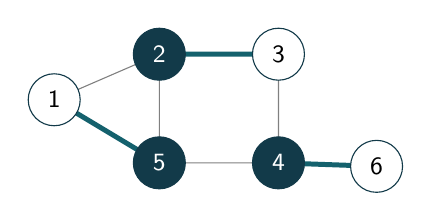
\begin{tikzpicture}[x=0.89cm,y=0.89cm,ordinary/.style={circle,draw=ink,fill=white,minimum size=6.6mm,inner sep=0.3pt,font=\small\sffamily},cover/.style={ordinary,fill=ink,text=white}]
\coordinate (a) at (0,0.9); \coordinate (b) at (1.5,1.55); \coordinate (c) at (3.2,1.55);
\coordinate (d) at (3.2,0); \coordinate (e) at (1.5,0); \coordinate (f) at (4.6,-0.05);
\draw[gray] (a)--(b)--(e)--(d)--(c);
\draw[linkcol,line width=1.8pt] (a)--(e) (b)--(c) (d)--(f);
\node[ordinary] at (a){1}; \node[cover] at (b){2}; \node[ordinary] at (c){3};
\node[cover] at (d){4}; \node[cover] at (e){5}; \node[ordinary] at (f){6};
\end{tikzpicture}\par
{\small Filled vertices give the cover. The three heavy edges give the matching.}
\end{center}
\end{example}\end{minipage}\par

\section{Paths, components and trees}
\label{stpaths}
Use vertices $0,\ldots,n-1$ and edge labels $0,\ldots,m-1$. An edge has two endpoint entries. In a directed graph they are read in tail--head order. Even parallel edges have distinct labels. A walk of length $k$ is an alternating table $v_0,e_1,v_1,\ldots,e_k,v_k$ obeying the incidence and, when appropriate, direction tests. A path has distinct vertices. A trail has distinct edges. A cycle is a nonempty closed trail with distinct vertices before its return. Thus a loop is a cycle of length one, and two parallel undirected edges give a cycle of length two. A walk of length zero has one vertex. All index searches below choose the first eligible index, with a separate failure flag.

\begin{theorem}[Reachability, shortest paths and separation]\leavevmode\label{stshort}
For vertices $s,t$, the existence of any walk from $s$ to $t$ is equivalent to the existence of a path of length at most $n-1$. One can return either a shortest path or a vertex set $S$ containing $s$, excluding $t$, and closed under every allowed step. With nonnegative integer edge weights one can likewise return a path of minimum total weight among all walks.
\end{theorem}
\begin{proof}
If $v_i=v_j$ for $i<j$, remove the subwalk from position $i$ to position $j$, retaining its common endpoint. Adjacency at the join holds even for directed edges. The endpoints are preserved, the length drops, and the total weight cannot increase. Given an input walk of length $k$, do this $k$ times, freezing whenever no repetition remains. At each step the resulting table is a walk with the specified endpoints and either it has stabilized or its length has fallen by at least the number of active steps. The output is a path. A repetition-free list of vertices has length at most $n$ because each newly marked vertex increases the cardinality of its $n$-bit mask by one. This also proves the bound for $s=t$, when the path has length zero.

For a direct decision procedure, start with $R_0=\{s\}$ and put $R_{i+1}=R_i\cup\{v:\text{a step }u\to v\text{ has }u\in R_i\}$. The equality with the endpoints of walks of length at most $i$ follows by removing or adding the last step. This induction quantifies only over tables of bounded length for its current $i$. On a vertex's first appearance after round zero, store a witnessing predecessor vertex and edge from the preceding round. Following these entries strictly lowers the first round and yields a path. If there were a shorter walk, the vertex would have appeared earlier. The shortening argument shows that $R_{n-1}$ contains every reachable vertex and hence is closed under a step. If it omits $t$, it supplies the required set. For nonnegative weights, minimize first the weight and then the length over the finite set of eligible paths. The erasure procedure applied to any competing walk proves optimality. One may enumerate the two tables of a walk of length $k$ by integers below $(n+1)^{k+1}$ and $(m+1)^k$. All minima have a candidate when the reachability decision succeeds.
\end{proof}

\begin{corollary}[Components, metric and condensation]\leavevmode\label{stcond}
Undirected reachability is an equivalence relation. Inside each component the unweighted shortest-path distance is a metric, and its diameter is at most the number of vertices in the component minus one. In a directed graph mutual reachability is an equivalence relation. Contracting its classes and omitting internal arcs produces a directed acyclic graph, which admits a topological ordering. A topological ordering exists precisely when a directed graph has no directed cycle.
\end{corollary}
\begin{proof}
Use the length-zero walk, reversal for undirected graphs, and concatenation followed by erasure. Mutual reachability uses a walk in each direction. Assign to each vertex the least mutually reachable vertex (the least reachable vertex in the undirected case). Equality of the resulting labels expresses class membership. For distance, length zero forces equal endpoints, reversal preserves length, and concatenating shortest paths gives the triangle inequality. A shortest path uses distinct vertices of its own component.

A directed cycle of distinct classes would make any two successive classes mutually reachable: lift each arc to an original arc, and connect its head to the tail of the next arc by a path inside their common class. This contradicts their distinct representatives. For a topological order, repeatedly remove the least remaining vertex with no incoming arc from a remaining vertex. If a nonempty remaining set had no such vertex, start at its least element and follow an incoming arc backwards $n$ times. Among the resulting $n+1$ vertices there is a repetition. Choose a repeated interval of minimal positive length. In the forward direction it is a directed cycle. The algorithm therefore removes all vertices of an acyclic graph in $n$ rounds, and each arc's tail must precede its head. Conversely a directed cycle would give a strictly increasing sequence of positions returning to its initial value. Every intermediate assertion can be checked on the remaining mask and the list of removed vertices. This gives either an order or an explicit cycle.
\end{proof}

\begin{corollary}[Transitive reduction and enumeration of directed acyclic graphs]\leavevmode\label{stdagenum}
For a finite simple directed acyclic graph, positive-length reachability is a strict partial order. Keeping its cover relations gives the unique inclusion-minimal subgraph with the same reachability. A topological ordering is unique exactly when the graph has a directed path through all its vertices (for $n\ge1$). The number $a_n$ of directed acyclic graphs on $n$ fixed labels satisfies $a_0=1$ and, for $n>0$,
\[
 a_n=\sum_{k=1}^{n}(-1)^{k-1}\binom nk 2^{k(n-k)}a_{n-k}.
\]
\end{corollary}
\begin{proof}
Write $u<v$ when a positive walk leads from $u$ to $v$. Concatenation gives transitivity, and a positive closed walk contains a directed cycle by the shortest-repetition argument. Keep $u\to v$ when $u<v$ and there is no $z$ with $u<z<v$. A walk witnessing such a pair must have length one. For an arbitrary comparable pair, start with its two-element chain and repeatedly insert an intermediate vertex in a gap where possible. A strict chain has at most $n$ vertices. The resulting saturated chain joins the pair using only retained edges. Every subgraph with the same reachability must retain each covering edge, because a longer path would exhibit an intermediate vertex. This proves uniqueness. In a topological order, every consecutive pair either has an arc in forward order or can be swapped: in the absence of this arc their interchange preserves every arc inequality. A unique order must therefore give a spanning directed path. Conversely that path forces the positions of all vertices in any order.

For the count, a nonempty acyclic graph has a source (no incoming arc), by the predecessor argument above. For a specified set of $k$ forced sources there are no arcs among them or entering them, and the $k(n-k)$ arcs leaving them for the complement are independent choices. The complement must induce one of the $a_{n-k}$ acyclic graphs. This already suffices for global acyclicity. Sum the forced-source counts with sign $(-1)^{k-1}$ over nonempty subsets of labels. A graph whose source set has $h>0$ elements receives total coefficient one: over all subsets, toggling the least source pairs equal numbers with opposite signs, and removing the empty term leaves the claimed coefficient for the chosen signs. Arithmetic with signs can again be expressed by an equality of natural sums. The graph masks enumerated have at most $n(n-1)$ bits.
\end{proof}

\begin{theorem}[Spanning forest and bridges]\leavevmode\label{stforest}
Let $c$ count the components, including isolated vertices. One can construct a spanning forest $F$ with exactly $n-c$ edges and the same components as the graph. In an undirected multigraph an edge is a bridge (its deletion increases $c$) exactly when it lies on no cycle. Deleting a bridge increases $c$ by one.
\end{theorem}
\begin{proof}
Start with all vertices, no edges. Scan the $m$ labels. Accept an edge precisely when its endpoints belong to different components of the accepted graph. Such an edge merges those two components and no others: a path using it splits into old walks on either side, and any two vertices in the merged blocks can be joined by using the new edge once. A cycle through the new edge would yield an old path between its endpoints by deleting it. Thus the accepted graph remains acyclic. A rejected edge already has a path between its endpoints, including the empty path for a loop. Consequently every scanned edge has connected endpoints in the accepted graph, and replacing the edges of any walk by these paths proves equality of the two reachability relations for the scanned prefix. The invariant $|F|+c_{F}=n$ starts with $n$ singleton blocks. Acceptance adds one on the left and removes one block. This proof includes the graph with $n=m=0$.

For an edge $e=uv$, compute connectivity in $G-e$. If a path from $u$ to $v$ survives, joining it to $e$ gives a cycle (a loop if $u=v$). Every transit that formerly used $e$ can use the path instead. Hence the component count is preserved. If there is no such path, adding $e$ back merges exactly two blocks as above. Any cycle containing it would have supplied the missing path.
\end{proof}

\begin{theorem}[Tree characterizations and leaves]\leavevmode\label{sttree}
For a nonempty finite undirected graph, each of the following four conditions characterizes a tree: (i) connected and acyclic, (ii) connected with every edge a bridge, (iii) connected with $n-1$ edges, and (iv) acyclic with $n-1$ edges. In a loopless graph these are also equivalent to having exactly one path between each pair of distinct vertices. A tree on at least two vertices has at least two leaves. Every nonempty subgraph of a forest has a vertex of degree at most one.
\end{theorem}
\begin{proof}
The spanning forest has $n-c$ edges. A rejected edge together with its forest path gives a cycle. Thus in an acyclic graph every edge belongs to the forest, and $m+c=n$. For a connected graph $c=1$, so equality $m=n-1$ forces every edge into the forest. The bridge criterion gives the second characterization.

Two different paths from $u$ to $v$ have a longest common initial segment (read edge labels as well as vertices). From its last vertex $z$, follow the first path up to its first subsequent intersection with the remainder of the second. Such an intersection exists at $v$. The two segments between $z$ and this intersection have different first edges and disjoint interiors. They form a cycle. Conversely, either arc of a loopless cycle gives a different path between the endpoints of any of its edges (one arc is that edge). Excluding loops in this characterization matters even for a single vertex.

In a tree with an edge, choose a longest path by bounded search. At either endpoint a second incident edge must either extend the path to a new vertex or close a cycle to a vertex already on it, with parallel edges included in the latter case. Both are impossible, so the distinct endpoints are leaves. In a nonempty subgraph of a forest apply this argument to any component containing an edge, or take an isolated vertex when there are no edges.
\end{proof}

\begin{corollary}[Paths, cycles and the degree profile]\leavevmode\label{stprofile}
A connected finite simple graph with exactly two vertices of degree one and all others of degree two is a path graph. A nonempty connected finite simple graph in which every vertex has degree two is a cycle graph. The converse holds for paths on at least two vertices and for cycles on at least three. In a tree on at least two vertices, the leaf count is
\[
  2+\sum_{v:\,d(v)\ge3}(d(v)-2).
\]
\end{corollary}
\begin{proof}
In the first graph the degree sum is $2n-2$. Each edge contributes two, so $m=n-1$ and the graph is a tree. A longest path has two leaf endpoints. A vertex outside it would have a first point of attachment reached along a path from outside. An internal attachment would have degree at least three, and an endpoint attachment would extend the path. Any extra edge on the path would form a cycle. In the second graph choose a longest path. Its first endpoint has a second neighbor on the path, closing a cycle. Every vertex on that cycle has already used both incident edges, and connectivity forbids outside vertices. Simplicity gives cycle length at least three. The converse degree lists follow by reading the defining edge sequences. For the displayed identity count the endpoints of all $n-1$ edges of the tree. Subtracting $2$ per vertex from $2(n-1)$ gives $-2$. Degree-one vertices contribute $-1$, degree-two vertices zero, and the other terms give the displayed sum. This signed identity can equivalently be read after moving all negative terms across the equality.
\end{proof}

\begin{theorem}[Minimum spanning forest]\leavevmode\label{stkruskal}
For natural edge weights, scanning edges in increasing order of $(\text{weight},\text{label})$ in Theorem~\ref{stforest} returns a minimum-total-weight spanning forest among those with the same components as the input. If all weights are distinct, it is the unique minimum forest.
\end{theorem}
\begin{proof}
Enumerate the $2^m$ subsets once to choose a minimum forest $T$. Existence follows from Theorem~\ref{stforest}. Maintain a minimum forest containing the accepted edges so far. When the next accepted edge $e=uv$ is absent from $T$, the unique $u$--$v$ path in $T$ leaves the current accepted component of $u$ along some edge $f$. This edge is outside the accepted forest. Every earlier scanned edge has endpoints in the same accepted component, so $f$ occurs later in the order and $w(e)\le w(f)$. Remove $f$ from $T$. Its component splits into two pieces separating $u,v$, since the old path was unique. Inserting $e$ reconnects these pieces without a cycle. The resulting forest still contains the previous accepted edges, now contains $e$, and costs no more, so it is minimum. At termination both forests contain $n-c$ edges, hence coincide. For distinct weights the exchange would strictly improve any minimum forest omitting $e$. Inducting through the scan with any proposed minimum forest proves uniqueness. The scan uses bounded selection sort, and the exchange family uses only edge masks.
\end{proof}

\section{Binary cycle and cut spaces}
\label{stspaces}
Identify an edge subset with its $m$-bit string. Addition is bitwise exclusive-or, denoted $\oplus$. Its scalar product with another string is the parity of the intersection size. For an edge mask $X$, its boundary $\partial X$ is the vertex mask of odd degrees in $X$. For a vertex mask $S$, the cut $\delta S$ contains edges whose two endpoint bits differ. A loop has zero boundary and belongs to no cut. The \emph{cycle space} consists of masks $X$ having $\partial X=0$. The \emph{cut space} consists of the $\delta S$. Both are closed under $\oplus$ by the endpoint formulas.

\begin{theorem}[Bases, dimensions and orthogonality]\leavevmode\label{stbases}
In an undirected multigraph with $n$ vertices, $m$ edges and $c$ components, a spanning forest gives explicit bases for the cycle and cut spaces, respectively of dimensions $m-n+c$ (read as $m-(n-c)$) and $n-c$. Each space is the orthogonal complement of the other.
\end{theorem}
\begin{proof}
Fix the spanning forest $F$. For each $e\notin F$, let $C_e$ consist of $e$ and the unique forest path joining its endpoints (empty for a loop). This is an even mask containing exactly one nonforest edge, namely $e$. For an even $X$, add $C_e$ for each nonforest edge $e$ marked in $X$. The resulting mask is even and supported in $F$. If it contained any edge, its nontrivial tree component would have a leaf of degree one by Theorem~\ref{sttree}, a contradiction. Hence it is zero. The coordinates of $X$ in this expansion are uniquely forced by its nonforest entries. This proves directly that the even masks are exactly the sums of cycles.

For each forest edge $f$ let $S_f$ be the component of its first endpoint in $F-f$ and put $D_f=\delta S_f$. Its only forest edge is $f$. If $\delta S$ is any cut, add $D_f$ for the forest edges it contains. The result is still a cut because $\delta S\oplus\delta T=\delta(S\oplus T)$. Its vertex-side indicator must be constant along every tree edge and hence on each component of $F$. Every graph edge stays within such a component. The resulting cut is empty. Again the forest entries give both the expansion and its uniqueness. There are therefore exactly $2^{m-(n-c)}$ cycle-space masks and $2^{n-c}$ cut-space masks, including zero in each count.

The parity of $|X\cap\delta S|$ equals that of $\sum_{v\in S} d_X(v)$, since internal edges contribute twice. Thus every even mask is orthogonal to every cut. Orthogonality to singleton cuts forces all degrees even. For the reverse direction, suppose $Y$ is orthogonal to every $C_e$. Form the cut $Z=\bigoplus_{f\in F\cap Y}D_f$. Then $Y\oplus Z$ vanishes on $F$ and is orthogonal to every $C_e$. Taking its product with $C_e$ reads just its $e$-bit, so all its other bits vanish too. This produces the desired cut equal to $Y$.
\end{proof}

\begin{corollary}[Prescribed odd vertices]\leavevmode\label{stboundary}
There exists an edge mask with boundary $T$ precisely when $T$ has even size in each component. In that case there are exactly $2^{m-(n-c)}$ such masks, and precisely one is supported in a fixed spanning forest.
\end{corollary}
\begin{proof}
Counting incidence ends within one component proves necessity. In each component with an even list of marked vertices, pair them in increasing order, join each pair by its forest path, and add the path masks modulo two. Each path has precisely its endpoints in its boundary, so the resulting forest mask $J$ has boundary $T$. Every other solution differs from $J$ by an even mask and conversely. An even mask contained in a forest is empty, as in the preceding proof. Component pairs and forest paths are bounded lists. Both the construction and its inverse on each fiber are explicit.
\end{proof}

\section{Euler tours and route inspection}
\label{steuler}
The \emph{support} of a graph is the set of vertices incident with at least one edge. Connectivity on the support ignores isolated vertices. In a directed graph, weak connectivity means connectivity after forgetting orientations, retaining the arc labels. A tour is a closed trail traversing every edge once.

\begin{theorem}[Undirected and directed Euler criterion]\leavevmode\label{steulertheorem}
Assume there is at least one edge. An undirected multigraph has a tour exactly when its support is connected and all degrees are even. It has an Euler trail from distinct specified vertices $a$ to $b$ exactly when its support is connected and the set of odd vertices is $\{a,b\}$. A directed multigraph has a tour exactly when its support is weakly connected and each vertex has equal in- and outdegree. For an open directed Euler trail from $a$ to $b$ the degree requirement is one extra outgoing arc at $a$, one extra incoming arc at $b$, and equality elsewhere. A tour may start at any support vertex.
\end{theorem}
\begin{proof}
A trail visiting every edge connects its support weakly. Count an arrival and a departure at every internal position, treating a loop as one of each. The excess degrees at the ends give precisely the stated necessity conditions for a directed walk. Forgetting direction pairs the incidence ends at internal positions and gives the undirected parity conditions.

Consider first either closed case. Start at a prescribed support vertex $r$. Traverse the least unused allowable edge out of the current vertex until stuck, with fuel $m$. In the undirected case, if the terminal vertex differed from $r$, its used incidence count would be odd. Its original incidence count is even, so an unused incident edge would remain. In the directed case a terminal vertex different from $r$ has received one more used arrival than used departure. Original balance forces at least one unused outgoing arc there. Thus the trail closes at $r$. It traverses at least one edge, since $r$ is incident and balance gives an outgoing arc in the directed case. Subtracting this closed trail leaves even degrees or equal in- and outdegrees in the residual graph, respectively.

If unused edges remain, some vertex of the current tour is incident with an unused edge. Indeed choose an unused edge, take a weak path from the tour to one of its ends, and if this end lies outside the tour inspect the first edge leaving the tour's vertex set. Such an edge is unused because both ends of every used edge occur on the tour. In the directed case residual balance supplies an unused outgoing arc even if the first incidence located is incoming. Apply the same traversal to the unused edges at that tour vertex and insert the resulting nonempty closed trail at its occurrence. The new trail is closed and repeats no label, since its two parts have disjoint edge masks. After $m$ possible rounds, freezing when finished, every label has been used. Each traversal and each insertion processes at most $m$ edges. The Boolean invariant checks closure and label uniqueness of the stored table, equality of its used mask with the set of its entries, and residual parity or balance. It also checks that the mask size increases on each active round.

In the open case add one new labelled edge between $b$ and $a$, directed $b\to a$ for the directed variant. The augmented graph satisfies the closed criterion. In its cyclic list locate the new edge and cut immediately after it, deleting it. The remaining trail goes from $a$ to $b$. Reverse it in the undirected case if necessary. The artificial edge never collides with an original label. If $m=0$, the only trails are length-zero trails at individual vertices, giving a tour precisely when $n>0$ under the walk convention above.
\end{proof}

\begin{corollary}[K\"onigsberg and cycle decomposition]\leavevmode\label{stkonigsberg}
The historic seven-bridge graph has no Euler trail. Any undirected even graph is a union of edge-disjoint cycles, as is any balanced directed graph (with directed cycles).
\end{corollary}
\begin{proof}
The four land masses have degrees $5,3,3,3$. The criterion allows at most two odd vertices. For the decomposition, take an Euler tour separately in each nontrivial weak component. In a nonempty closed trail find a shortest positive interval with equal endpoint vertices. Its intervening vertices are all distinct and its edges are already distinct, so it is a cycle. Delete it and splice at the common vertex. The remainder is a closed trail, possibly empty. Each deletion uses at least one previously unassigned edge, and $m$ rounds suffice.
\end{proof}

\begin{theorem}[Undirected route inspection]\leavevmode\label{stpostman}
Let the support be nonempty and connected, with natural edge weights $w$. Write $T$ for its odd vertices, $W$ for the sum of all edge weights, and $d(u,v)$ for shortest weighted distance. The minimum cost of a closed walk traversing every edge at least once equals
\[
 W+\min_P\ \sum_{\{u,v\}\in P}d(u,v),
\]
where $P$ pairs all vertices of $T$. The empty pairing has cost zero. Both a minimizing pairing and an optimum walk are primitive-recursive outputs.
\end{theorem}
\begin{proof}
$T$ has even size, since the sum of degrees is $2m$. Enumerate pairings (for example all permutations of its increasing list, pairing consecutive entries). Take shortest paths for the pairs in a minimizing pairing, and add a fresh copy of every edge occurrence on those paths. This adds odd degree exactly at $T$, so the Euler criterion yields a tour in the resulting multigraph. Reading its new labels as their original edges attains the displayed cost. The number of edge copies added is at most $(|T|/2)(n-1)$.

Conversely, take any closed covering walk and reserve one occurrence of each original edge. The remaining occurrence multigraph $H$ has odd vertices exactly $T$, because the whole occurrence multigraph is even. Add a fresh vertex $z$ and one new edge from $z$ to each member of $T$. This graph is even. If $T\ne\varnothing$, take an Euler tour of the component containing $z$, starting at $z$. Delete the new edges and split the tour at its visits to $z$. Each excursion from $z$ pairs two distinct vertices of $T$, because each such vertex has just one added edge. Its intervening edges form a walk in $H$. Each member of $T$ occurs in exactly one pair. The total weight of these walks is at most the weight of $H$, even when $H$ has additional disjoint components. Each walk costs at least its endpoint distance, proving the lower bound. For empty $T$ the lower bound follows directly from nonnegativity. An arbitrary competitor is a finite input table. The lower-bound argument uses loops bounded by its own length, whereas the optimum constructor uses only the original graph and weights.
\end{proof}

\section{Counting labelled trees and rooted forests}
\label{stcounttrees}
\begin{theorem}[Pr\"ufer coding and Cayley's formula]\leavevmode\label{stprufer}
For $n\ge2$, labelled simple trees on $\{0,\ldots,n-1\}$ correspond bijectively to words of length $n-2$ over that alphabet. A vertex $v$ occurs exactly $d(v)-1$ times in its tree's word. Thus there are $n^{n-2}$ such trees. For prescribed positive degrees $d_v$ with $\sum_v d_v=2(n-1)$, their number is the multinomial coefficient
\[
  \frac{(n-2)!}{\prod_v(d_v-1)!}.
\]
There is one tree on a single labelled vertex.
\end{theorem}
\begin{proof}
To encode, remove the least leaf and record its unique neighbor, until two vertices remain. A leaf exists at each step by Theorem~\ref{sttree}. Deleting it leaves a tree: no path between two remaining vertices can pass through a leaf internally. A vertex begins with $d(v)$ incident edges. Each time an incident edge is removed before that vertex becomes a removed leaf, its neighbor was removed and this vertex was recorded. At its removal it has one edge left, and the two final vertices also have one edge left. This proves the occurrence count, including for the tree remaining at every intermediate stage.

Decode by starting with all labels active. At a stage with $k>2$ active vertices, the remaining suffix has length $k-2$ and uses only active labels. The least active label $p$ absent from the suffix exists, by marking its entries. Join $p$ to the first letter $q$, delete $p$ from the active set, and drop that first letter. Since $q$ occurs, $q\ne p$, and the invariant on active labels persists. At $k=2$ join the last two labels. Reading the operations backwards starts with a single edge and repeatedly attaches a fresh leaf, so the output is a tree. At any decoding stage, the tree made by this suffix has degree at each active label equal to one plus its multiplicity in the suffix: the last two vertices start at one, and reinserting $p$ of multiplicity zero increases the degree only of $q$, whose missing occurrence was exactly the dropped letter. Hence encoding this reconstructed tree removes precisely the decoder's least absent label and writes $q$. In the other direction the occurrence count for every residual encoded tree makes its least leaf precisely the decoder's next choice, so decoding recovers all removed edges and the last edge. Both inverse identities use at most $n$ transitions. The prescribed degree formula counts words with those multiplicities: choose disjoint position sets of the required sizes in increasing vertex order. The product of successive binomial coefficients times $\prod_v(d_v-1)!$ equals $(n-2)!$ by cancellation, giving the integer quotient displayed.
\end{proof}

\begin{theorem}[Weighted matrix--tree and rooted-forest identities]\leavevmode\label{stkirchhoff}
Orient the edges of an undirected labelled multigraph arbitrarily, and let $B$ be its signed incidence matrix, with column $e$ equal to the unit vector at its tail minus the one at its head. A loop gives zero. For natural weights $w_e$, put $L=B\,\mathrm{diag}(w_e)\,B^{\mathsf T}$. For a set of roots $R$ delete its rows and columns, leaving $L_{\bar R,\bar R}$. Then
\[
 \det L_{\bar R,\bar R}=
 \sum_{F}\ \prod_{e\in F}w_e,
\]
where the sum ranges over spanning forests having exactly one root per component. With one specified root this is the spanning-tree count with weights. At unit weights every principal cofactor of a nonempty graph counts the spanning trees. As usual a $0$-by-$0$ determinant and an empty product equal one.
\end{theorem}
\begin{proof}
We first prove the finite determinant identity needed here. For a $k$-by-$m$ matrix $U$ and an $m$-by-$k$ matrix $V$, expand the determinant of $UV$ by permutations, then expand each factor $(UV)_{i,\sigma(i)}$ by its inner index. Grouping terms by the list of indices $h(1),\ldots,h(k)$ gives
\[
  \det(UV)=\sum_{h:[k]\to[m]}
    \left(\prod_i U_{i,h(i)}\right)
    \det\big(V_{h(i),j}\big)_{i,j\in[k]} .
\]
Here $[k]$ denotes an index set of size $k$. If $h$ repeats an index, the inner determinant has equal rows. Terms in its permutation sum cancel in pairs by swapping the columns assigned to those two rows. Otherwise write the image as an increasing list $S$ and $h(i)=S_{\pi(i)}$. The inner determinant is then $\operatorname{sgn}(\pi)\det V_{S,:}$ by permuting rows. Summing over $\pi$ gives precisely $\det U_{:,S}\det V_{S,:}$. Thus the sum over all $k$-element subsets $S$ gives $\det(UV)$, including $k>m$ when it is zero. The sign rules here follow from inversion parity: swapping two positions changes it by an odd number (one for that pair plus an even contribution from intermediate entries), and sorting a permutation by swaps proves the row-permutation rule. Equal columns, column linearity, Laplace expansion along a row with one nonzero entry, and invariance under transposition likewise follow from the permutation formula: group by the assigned column in a given row, or replace a permutation by its inverse for transposition.

Put $A=B_{\bar R,:}$ and $k=n-|R|$. The identity with $U=A\,\mathrm{diag}(w)$ and $V=A^{\mathsf T}$ gives one summand $(\prod_{e\in S}w_e)\det(A_{:,S})^2$ per $k$-edge subset. If $S$ contains a cycle, its columns around that cycle, signed according as the orientation agrees with the traversal, sum to zero. For a loop the one column is zero. Solve this relation for one column, expand linearly, and each term has a duplicate column or is zero. Thus its determinant vanishes.

If $S$ is a forest, it has $n-k=|R|$ components. A component without a root supplies a nonempty family of retained rows whose sum is zero, because each selected edge contributes opposite ends within its component. The same linearity argument forces determinant zero. Otherwise each component has exactly one root by counting. When $k>0$ there is a nontrivial component. Its two or more leaves include at least one nonroot leaf $v$. Its row has a single entry $+1$ or $-1$. Expanding there deletes that vertex and its edge, with all root conditions preserved, and changes the determinant only by a sign. Repeating $k$ times leaves the empty determinant, proving the squared determinant is one. The argument also covers $R=\varnothing$: a nonempty forest cannot have zero components, and the empty graph contributes its empty forest.
\end{proof}

\begin{corollary}[Rooted-forest generating function and directed trees]\leavevmode\label{stforestgen}
For a natural number $t$,
\[
 \det(tI+L)=\sum_F t^{c(F)}\left(\prod_{C\text{ component of }F}|C|\right)
                      \left(\prod_{e\in F} w_e\right),
\]
with $F$ now ranging over all spanning forests. For a weighted directed multigraph the principal minor with roots $R$ of its outdegree Laplacian counts, with product weights, spanning directed forests whose arcs lead to exactly one root in each component.
\end{corollary}
\begin{proof}
Expand by choosing in each column either the $tI$ column or the $L$ column. For the set $R$ of identity columns, the corresponding permutations fix $R$ and contribute $t^{|R|}\det L_{\bar R,\bar R}$: deleting fixed points does not change permutation sign, as is seen from its disjoint cycles or by simultaneous row and column permutation. Apply Theorem~\ref{stkirchhoff}. Given $F$, choosing one root independently in each component gives the product of component sizes.

In the directed case put $H_{v,e}=1$ when $v$ is the tail of $e$, zero otherwise, and take $B$ with the given arc orientations. The outdegree Laplacian is $H\,\mathrm{diag}(w)\,B^{\mathsf T}$, with a loop cancelling in its diagonal entry. Apply the same product identity to the retained rows. The $B$ minor is nonzero exactly when the chosen arcs form an underlying forest with one root per component, as proved above. The $H$ minor is nonzero precisely when each retained vertex is the tail of exactly one chosen arc and no root is a tail, because its columns must be distinct retained unit vectors. In such a forest, following the outgoing arc strictly advances toward the root: iteration must stop at a root, since a repeat would be a directed cycle, including a two-edge cycle if applicable. To compute the product of minor signs, order the vertices by decreasing distance from their roots and put the columns in the corresponding tail order. Then $H$ becomes the identity, and $B$ is triangular with diagonal $1$ (the other entry, if retained, is in the parent's later row). Simultaneous reordering changes both determinants by the same sign. Their product is therefore $+1$, which proves the formula.
\end{proof}

\begin{corollary}[Last-exit trees count Euler tours]\leavevmode\label{stbest}
Let a finite directed multigraph have nonempty weakly connected support, equal in- and outdegrees, and distinguished vertex $r$ on the support. Work on that support and write $d(v)$ for outdegree, $\tau_r$ for the number of spanning directed trees pointing towards $r$. Fix an outgoing arc $b$ at $r$. The number of ordered lists of all labelled arcs forming tours starting with $b$ is
\[
       \tau_r\prod_v (d(v)-1)! .
\]
Allowing any first arc at $r$ multiplies this by $d(r)$. The directed minor in Corollary~\ref{stforestgen} computes $\tau_r$.
\end{corollary}
\begin{proof}
Read a tour as a list of departures at each vertex in temporal order. For every $v\ne r$ mark its last departure. If it leads to $u\ne r$, the tour must leave $u$ later, since its final vertex is $r$. Thus the times of marked departures would strictly increase around any directed cycle of marks. Each nonroot vertex has one mark and every mark sequence ends at $r$ within $n$ steps. The underlying marked graph is connected and has one fewer edge than vertices, hence is a tree. The marked arcs point towards $r$.

Conversely choose such a tree. At each nonroot vertex order its departures arbitrarily with its tree arc last. At $r$ order the departures with $b$ first. Start at $r$ and on each visit take the first unused arc in the prescribed local list. By balance it can stop only at $r$, as in Theorem~\ref{steulertheorem}. At this point the used trail is closed, so unused indegree and outdegree agree everywhere. If some vertex has unused departures, it is a nonroot and its last arc is unused. Its parent now has an unused incoming arc, hence an unused departure. Following parents in the tree forces an unused departure at $r$, contradicting termination. Hence this procedure recovers a tour, and its recorded local lists and tree are the choices used to generate it. Each local order with its one prescribed end or beginning has $(d(v)-1)!$ possibilities with distinct arc labels. This proves the product and supplies mutually inverse bounded algorithms.
\end{proof}

\paragraph{Arithmetic implementation.}
Determinants above are finite signed sums indexed by permutation tables. Integers may be stored as pairs of naturals with equality by cross-addition. Compute sign by inversion-count parity. For a matrix of order $k$ with entries of absolute value at most $M$, the sum of absolute values of its permutation terms is at most $k!(M+1)^k$. A forest certificate consists of an $m$-bit mask, the endpoint table, and an $n$-bit root mask. All assertions about minors in the leaf-stripping argument concern explicitly computed matrices. Fix the original graph and enumerate submasks of its row and column masks (at most $2^{n+m}$ possibilities). Induct on the number of retained rows using the Boolean conjunction of the minor statement for all relevant submasks of that size, keeping the original indexing of all survivors. This provides the smaller instance after leaf removal using quantifier-free induction. The permutation and map expansions are double finite folds and their regroupings are witnessed by sorting index lists. Pr\"ufer coding uses at most $n$ steps and suffixes of a single word. Its backward invariant is the active-vertex mask together with its degree vector and suffix multiplicity vector. Both are computed by bounded folds. These give direct targets for Lean definitions and induction statements.

\section{Graph operations, symmetry, and enumeration}\label{sec:ops}
\begin{proposition}[Products and line graphs]\leavevmode\label{prop:products}
Suppose $G,H$ are simple, with orders $n,h$, sizes $m,l$, and degrees $d_u,e_x$.
The following counts hold, with product vertices $(u,x)\in[n]\times[h]$.
\[
\begin{array}{lcc}
\toprule
\text{graph} & \text{degree at }(u,x)&\text{number of edges}\\
\midrule
G\square H &d_u+e_x&mh+ln\\
G\times H &d_u e_x&2ml\\
G\boxtimes H&d_u+e_x+d_u e_x&mh+ln+2ml\\
G[H]&h d_u+e_x&mh^2+nl\\
\bottomrule
\end{array}
\]
If both factors are nonempty and connected, Cartesian distance is the sum
of the factor distances. The line graph $L(G)$ has $m$ vertices and
$\sum_v\binom{d_v}{2}$ edges. Its vertex $uv$ has degree $d_u+d_v-2$.
\end{proposition}
\begin{proof}
In the Cartesian product change one coordinate along an edge, leaving the
other fixed. In the tensor product change both along edges independently.
Their disjoint union of neighbour lists is the strong product's neighbour
list. In the lexicographic product either change the first coordinate along
an edge, freely choosing the new second coordinate, or leave the first fixed
and move along an edge of $H$. These disjoint alternatives give the middle
column. Sum it over all $(u,x)$ and apply the handshaking identity to the two
factors for the right column. Any Cartesian walk projects to walks after
deleting stationary steps. Their lengths sum to the original length. Following
two shortest walks in succession realizes that lower bound. Two different
edges of a simple graph sharing a vertex share exactly one. Count pairs there,
or count the other edges at the two ends of a given $uv$.
\end{proof}

\begin{proposition}[Homomorphisms, subgraphs, and minors]\leavevmode\label{idx:operations-homomorphisms-subgraphs-and-minors}
A homomorphism is a table $f:[n]\to[h]$ sending edges to edges. Composition
preserves this condition, and $G$ has a $q$-colouring exactly when it admits
a homomorphism to $K_q$. A subgraph embedding is an injective edge-preserving
table, and is induced precisely when it also preserves nonedges at distinct
arguments. Isomorphism, containment as an ordinary or induced subgraph, and
minor containment are all decidable by PR procedures returning certificates.
\end{proposition}
\begin{proof}
Substitute the image of each edge into the next table. In $K_q$ two colours
are adjacent exactly when distinct. Scan all maps (at most $\max(2,h)^n$
codes), checking the desired row conditions. Isomorphism adds surjectivity
and reflection of adjacency, so its inverse is a bounded lookup. For a
minor of $G$ modelled on $H$, search for $h$ disjoint nonempty connected
branch sets in $[n]$, checking for a crossing edge for each edge of $H$.
Use codes below $2^{nh}$ and connectivity restricted to each mask. In an
actual sequence of deletions and contractions keep the sets of original
vertices represented by surviving vertices. Unions joined by an edge stay
connected, and every surviving edge has two original representatives in the
indicated sets. Conversely retain a spanning tree in each branch set and
one crossing edge for each required adjacency, delete everything else and
contract the retained trees. This constructs the minor and proves completeness
of the decision procedure.
\end{proof}

\begin{proposition}[Labelled, connected, and unlabelled graphs]\leavevmode\label{prop:burn}
Put $N=\binom n2$. There are $a_n=2^N$ labelled simple graphs on $[n]$,
$\binom Nm$ of size $m$, and $c_n$ connected graphs for $n\ge1$, where
\[
 c_n=a_n-\sum_{j=1}^{n-1}\binom{n-1}{j-1}c_j a_{n-j}.
\]
If $u_n$ counts isomorphism classes, and $o_2(\pi)$ counts cycles of $\pi$
on unordered vertex pairs, then
\[
 n!\,u_n=\sum_{\pi\in S_n} 2^{o_2(\pi)} .
\]
The numbers of loopless digraphs, oriented simple graphs and tournaments
on $[n]$ are respectively $4^N,3^N,2^N$.
\end{proposition}
\begin{proof}
The upper triangle has $N$ independent bits, and a mask of weight $m$ is
an $m$-subset. Pascal's recurrence counts it by splitting at the last slot.
For a nonempty graph choose the component of vertex zero. Its other labels
form a $(j-1)$-subset of $[n]\setminus\{0\}$, its induced graph is connected,
and the complement carries an arbitrary graph. Sorting either set supplies
a canonical labelling. The joining construction has no cross edges. The case
$j=n$ gives $c_n$, so the displayed subtraction is exact. For a fixed
permutation, an invariant graph chooses one bit for each orbit of pairs.
Count all $(\pi,G)$ with $\pi G=G$ by their graph or by their permutation.
Group the graph side using the least code in each orbit. For a representative
$R$, every orbit member $H$ has as many transporters $\pi R=H$ as stabilizers
of $R$: compose with the least transporter, which exists by finite search.
Its stabilizer has the same size as that of $H$, by conjugation. The fibres
over $H$ partition all $n!$ permutations, so each orbit contributes exactly
$n!$. Permutations are counted by successively selecting unused images.
Finally for each pair of labels the allowed directed states number four
(neither, either, both), three (exclude both) or two (exactly one).
\end{proof}

\begin{corollary}[Finite random graph counts and a Ramsey lower certificate]\leavevmode\label{idx:operations-finite-random-graph-counts-and-a-ramsey-lower-certifica}
In the uniform list of $2^N$ graphs the mean number of $k$-cliques for
$1\le k\le n$ is $\binom nk/2^{\binom k2}$. If
$2\binom nk<2^{\binom k2}$ there exists a graph on $n$ vertices with neither
a $k$-clique nor an independent $k$-set, and the least such mask is PR.
\end{corollary}
\begin{proof}
Fix the $k$ labels. Requiring every internal bit to equal one leaves
$2^{N-\binom k2}$ masks. Requiring zero leaves the same number. Count incidences
of a mask with a distinguished clique (or independent set) and sum over label
sets. Under the strict inequality the total number of incidences of either
kind is smaller than $2^N$. If every mask had at least one incidence the
sum would be at least $2^N$. A bounded scan therefore finds a zero count.
\end{proof}

\begin{theorem}[The Petersen graph]\leavevmode\label{thm:petersen}
Take the two-subsets of $[5]$ as vertices, with disjointness for adjacency.
This graph has order $10$, size $15$, diameter $2$, girth $5$, and strongly
regular parameters $(10,3,0,1)$. Its automorphism group is the full $S_5$
acting on the underlying labels, so it has order $120$. Its chromatic number
is three.
\end{theorem}
\begin{proof}
There are $\binom52$ vertices. For a fixed pair choose two of the remaining
three labels to find its three neighbours. Disjoint pairs use four labels
and have no common neighbour. Intersecting distinct pairs use three, leaving
exactly one common neighbour. These counts imply the diameter and exclude
triangles and four-cycles (opposite vertices of a four-cycle have two common
neighbours). With underlying labels $1,\ldots,5$, the sequence
$12,34,15,23,45,12$ is a five-cycle. An independent family consists of
pairwise intersecting pairs. If it contains $ab,ac$, every pair avoiding
$a$ must be $bc$, and no fourth distinct pair can meet all three of
$ab,ac,bc$. Thus the only independent families of size four are the five
full stars about a label. Automorphisms permute the stars, and the star
pair about $a,b$ intersects in the single vertex $ab$. Their action on
stars determines their action everywhere. Every permutation of the five
labels preserves disjointness, proving the group assertion. Colour the star
at label 1 first, the remaining pairs containing 2 second, and the three
pairs on $\{3,4,5\}$ third. Each class is intersecting. An odd cycle cannot
alternate two colours all the way round.
\end{proof}

\begin{proposition}[Intersection representation]\leavevmode\label{idx:operations-intersection-representation}
Every finite simple graph is an intersection graph of finite sets.
\end{proposition}
\begin{proof}
For the intersection representation, assign each vertex its set of incident
edge labels plus a private marker. Distinct vertices' sets intersect precisely
in their common edge if there is one. The markers distinguish isolated
vertices and leave all intersection tests between different vertices unchanged.
\end{proof}

\begin{theorem}[The graphic matroid and submodularity]\leavevmode\label{thm:matroid}
For a multigraph on $[n]$ the acyclic edge masks form a matroid: they contain
the empty mask, are closed under restriction, and if $I,J$ are acyclic with
$|I|<|J|$, one can extend $I$ by an edge of $J\setminus I$ while preserving
acyclicity. Its rank on $A$ is $r(A)=n-c(A)$, and
\[
 r(A\cup B)+r(A\cap B)\ \le\ r(A)+r(B).
\]
\end{theorem}
\begin{proof}
The first two assertions follow by the cycle test. If every edge of $J$ lies
inside the components of $I$, then in each such component, with $b$ vertices,
$J$ has at most $b-1$ edges because its restriction is a forest. Summing gives
$|J|\le n-c(I)=|I|$, contrary to the hypothesis. A crossing edge, found by
a scan, joins two components and creates no cycle. A maximal forest in $A$
spans exactly its components, giving the rank formula and a basis algorithm.
The increase in rank on inserting an edge equals one if its endpoints were
in different components and zero otherwise. For nested edge sets this
increment can only decrease on passage to the larger set. Start with
$A\cap B\subseteq B$ and insert, on both sides, the same successive edges
of $A\setminus B$. Adding the increment inequalities gives
$r(A)-r(A\cap B)\ge r(A\cup B)-r(B)$.
\end{proof}

\begin{theorem}[Reconstruction from the vertex-deleted deck]\leavevmode\label{thm:deck}
For a simple graph $G$ on $n\ge3$ vertices let its deck be the multiset of
unlabelled cards $G-v$. From the deck one can reconstruct the degree multiset,
counts of all smaller induced subgraph types, and, if $G$ is regular or
disconnected, the isomorphism type of $G$. Both special classes are recognizable.
\end{theorem}
\begin{proof}
Encode an unlabelled graph by the least adjacency mask among all its
relabellings. A card of order $n-1$ therefore has a canonically labelled
representative, with repetitions retained in the deck. For each graph $H$
of order $j<n$, write $s(H,G)$ for the count of $j$-vertex subsets inducing
$H$ up to isomorphism. A subset survives deletion in precisely $n-j$ cards,
so $(n-j)s(H,G)=\sum_v s(H,G-v)$. The same argument works for copies of
ordinary subgraphs on $j$ vertices. In particular the edge count $m$ is
the sum of the card edge counts divided by $n-2$, and $d(v)=m-|E(G-v)|$.
These divisions are exact by the counts. If the degrees all equal $d$,
choose any card. The neighbours of its missing vertex have degree $d-1$ there
and the other vertices degree $d$. Attach one vertex to the former group.
For $d=0$ simply add an isolated vertex.

A connected graph with at least two vertices has at least two connected
cards: removing either of two leaves of a spanning tree preserves the rest
of the tree. In a disconnected graph, a deletion can give a connected card
only if it removes an entire singleton component and exactly one component
then remains. For $n\ge3$ this can happen at most once. This recognizes
connectivity. In the disconnected case every component has order $<n$.
Consider all connected types $H$ of smaller order, in decreasing order of size,
and write $b_H$ for their unknown component multiplicities. A connected
induced copy of $H$ lies inside one component. Thus
\[
 b_H=s(H,G)-\sum_{\substack{C\ {\rm connected}\\|H|<|C|< n}}
                   b_C\,s(H,C).
\]
Among components of the same order an induced copy uses the whole component,
so only type $H$ contributes. Each difference is a nonnegative integer by
the counting identity. Their disjoint union reconstructs $G$. All types
can be listed by scanning masks up to $2^{\binom n2}$ and taking least codes.
This proves the stated special cases without a general reconstruction premise.
\end{proof}

\section{Prescribing the full automorphism group}\label{co:symmetry}
A graph automorphism is an adjacency-preserving permutation whose inverse
also preserves adjacency. A finite group is given by a multiplication
table on $[m]$ with $m\ge1$, an identity $1_G$ and an inverse table.
The group equations are finite tests. For each $a$ the permutation
$L_a(x)=ax$ has inverse $L_{a^{-1}}$ and satisfies $L_aL_b=L_{ab}$.
Evaluation at the identity distinguishes the translations. This already
proves Cayley's permutation representation theorem.

For a subset $S$ closed under inversion and excluding the identity,
join $x$ to $xs$ for each $s\in S$. The resulting simple undirected
Cayley graph has degree $|S|$ by cancellation. Left translations give
a transitive group of automorphisms. Its component at $1_G$ is exactly
the subgroup generated by $S$: a path spells a product of generators,
and any product gives a walk by its successive partial products. More
explicitly, the reachable mask at $1_G$ is closed under multiplication
and inversion by concatenating generator words and reversing them with
inverted letters. Translating it gives all the other components as left
cosets. Reachability needs paths of length at most $m-1$, so the component
description also computes subgroup membership.

\begin{theorem}[Finite Frucht realization]\leavevmode\label{co:frucht}
One can construct a connected simple undirected graph on at most
$(m+2m^2)(2m+2)$ vertices whose full automorphism group is isomorphic
to the given group. Both directions of the isomorphism are explicit.
\end{theorem}
\begin{proof}
Introduce a vertex $v_x$ for each group element $x$. For each ordered
pair $x,g$ use distinct new vertices $a_{x,g},b_{x,g}$ and the edges
of the walk
\[
 v_x\;--\; a_{x,g}\;--\; b_{x,g}\;--\; v_{xg}.
\]
When $g=1_G$ these three edges form a triangle. All are ordinary
edges of a simple graph, including when $m=1$. Call the vertices
introduced so far the core. At each core vertex attach a fresh path
by one endpoint. Its length is one at $v_x$, $2+2g$ at $a_{x,g}$,
and $3+2g$ at $b_{x,g}$, using $g\in[m]$ as its numerical label.
There are $m+2m^2$ core vertices and each attached path adds at most
$2m+1$ vertices. All core vertices can reach a $v_x$, and the walks
from $v_{1_G}$ reach every $v_x$. The graph is connected.

In the finished graph, core vertices are exactly those of degree at
least three: at each $a$ or $b$ there are two distinct core neighbours
and the attached path, and each $v_x$ has $2m$ distinct core neighbours.
All remaining vertices lie on paths and have degree one or two.
Each core vertex has exactly one noncore neighbour, and following the
unique attached path recovers its length. It follows that any automorphism
preserves the three types, including $g$ on both inner types. Write
$v_x\mapsto v_{\pi(x)}$. There is a unique neighbour of type $a_{*,g}$
at each $v_x$, so $a_{x,g}\mapsto a_{\pi(x),g}$. Its unique neighbour
of type $b_{*,g}$ then forces $b_{x,g}\mapsto b_{\pi(x),g}$. The
remaining core adjacency gives $\pi(xg)=\pi(x)g$. Substituting
$x=1_G$ proves $\pi=L_{\pi(1_G)}$. Images of all core vertices have now
been determined, and distances along their rooted paths force the images
of all other vertices.

Conversely each $L_z$ acts on the three core types by replacing $x$ by
$zx$ and preserving $g$. Associativity preserves the terminal incidence
at $v_{xg}$, and sending each path position to the same position on the
image path extends this to an automorphism with inverse indexed by $z^{-1}$.
The resulting automorphisms compose by group multiplication. Reading
the image of $v_{1_G}$ gives the inverse function on the full
automorphism group. Given the graph order bound $M$, all permutation and
inverse tests scan words of length at most $M$ with entries below $M$.
Core types and path lengths are recovered in at most $M$ steps.
\end{proof}

\section{Laplacian energy and exact spectral data}\label{sec:spectral}
We use the characteristic polynomial $p_M(t)=\det(tI-M)$, a finite coefficient table over the integers. A rational eigenpair is a rational scalar $\lambda$ and a specified nonzero rational vector $x$ with $Mx=\lambda x$. Vector entries may be cleared of denominators by multiplying by their product. All arithmetic and comparisons in the following arguments are finite.

\begin{theorem}[Laplacian energy, nullity and eigenvalue bounds]\leavevmode\label{spec:energy}
For an undirected multigraph with natural weights put $L=B\,\mathrm{diag}(w_e)\,B^{\mathsf T}$ as in Theorem~\ref{stkirchhoff}. On rational vertex vectors,
\[
 x^{\mathsf T}Lx=\sum_{e=uv} w_e(x_u-x_v)^2.
\]
The indicator vectors of the components of the positive-weight edges form a basis of the kernel (include isolated vertices). Thus zero has algebraic multiplicity equal to their number $c$. For a nonempty graph let $\Delta$ be the maximum sum of weights of nonloop incidences at a vertex. Every rational eigenvalue of $L$ is an integer in $[0,2\Delta]$. When the positive-weight graph is connected and $n\ge2$, every nonzero rational eigenpair satisfies $\lambda\ge 2/(n-1)^2$.
\end{theorem}
\begin{proof}
Entry $e$ of $B^{\mathsf T}x$ is the difference of its endpoint values. Expand the quadratic form by first summing over the edge index. A sum of nonnegative rationals vanishes precisely when all its terms vanish (clear denominators). Thus if $Lx=0$, each positive edge has equal endpoint values and so do the ends of every positive-edge path. Conversely any vector constant on the components satisfies $Lx=0$ by multiplication. Its component values supply unique coordinates in the asserted basis.

To obtain algebraic multiplicity directly, discard zero-weight edges, which contribute zero to $L$. In Corollary~\ref{stforestgen} every spanning forest has at least $c$ components. A spanning forest with exactly $c$ exists by Theorem~\ref{stforest}, and its root-count times edge-weight product is positive, including the empty graph convention. All coefficients are nonnegative, so the least nonzero power of $t$ in $\det(tI+L)$ is $t^c$. Replacing $t$ by $-t$ yields the assertion for $p_L$.

For an eigenpair, $x^{\mathsf T}Lx=\lambda\sum_v x_v^2$ has positive denominator sum $\sum_v x_v^2$. This proves nonnegativity. Since $(a-b)^2\le2a^2+2b^2$ by $(a+b)^2\ge0$, summing over nonloops proves the upper bound. For any integer matrix its characteristic polynomial is monic, by the permutation formula, and vanishes at a rational eigenvalue: in $\lambda I-L$ a nonzero eigenvector gives a linear dependence of the columns with a nonzero, hence invertible, rational coefficient. If $a/b$ in lowest terms, $b>0$, solves a monic polynomial, clearing denominators gives $b\mid a^n$. To see $b=1$, the Euclidean algorithm for $|a|,b$ gives a signed inverse to $a$ modulo $b$ when their gcd is one (each remainder is a combination of the previous pair, and each positive step decreases the divisor). Its $n$th power is inverse to $a^n$ there, so $b\mid1$. All divisions in this argument are bounded by the dividend and the coefficient computations use the same fixed recursion on the Euclidean steps.

For the lower bound, all column sums of $L$ vanish, hence $\lambda\ne0$ forces $\sum_v x_v=0$. Expansion gives $\sum_{u<v}(x_u-x_v)^2=n\sum_v x_v^2$. For each pair choose a simple positive-edge path of length $\ell\le n-1$. The squared telescoping sum of its endpoint differences is at most $\ell$ times the sum of their squares: subtract the first quantity from the second to obtain the sum of $(a_i-a_j)^2$ over unordered pairs of steps. Every path-edge weight is at least one. Writing $E=x^{\mathsf T}Lx$, we get $n\sum_v x_v^2\le\binom n2(n-1)E$, proving the bound after cancellation.
\end{proof}

\begin{theorem}[A bipartiteness test in the characteristic polynomial]\leavevmode\label{spec:bip}
For a finite simple graph with adjacency matrix $A$, the graph is bipartite exactly when $p_A(t)=(-1)^n p_A(-t)$. If the graph is nonbipartite, let $g$ be the length of its shortest odd cycle. The coefficient of $t^{n-g}$ in $p_A(t)$ is minus twice the number of undirected cycles of length $g$ (identified up to rotation and reversal). All coefficients of $t^{n-j}$ for smaller odd $j$ vanish.
\end{theorem}
\begin{proof}
A bipartition supplies a diagonal matrix $D$ with signs $+1,-1$ on the two classes. We have $DAD=-A$ and $D^2=I$. Determinant multiplicativity, the square-matrix case of the product formula proved in Theorem~\ref{stkirchhoff}, gives $p_A(t)=\det(tI+A)=(-1)^n p_A(-t)$.

For the converse, first produce an odd cycle whenever the graph fails the bipartition test. Colour each vertex by the parity of its depth in a rooted spanning forest. If some edge joins equal colours, follow the two root paths from their last common vertex to its endpoints and close along the edge. The two lengths have the same parity, and their paths are internally disjoint, so the resulting cycle is odd. A forest edge cannot be the offending edge. Bounded minimization gives $g$.

In the determinant expansion a permutation moving $j$ vertices contributes to $t^{n-j}$, since the diagonal entries are $t$ and all off-diagonal nonzero entries are $-1$. Every nontrivial permutation cycle of length at least three in a nonzero term follows a simple graph cycle. A transposition needs just one undirected edge. Odd $j$ requires an odd permutation-cycle length, at least $g$. For $j=g$ all moved vertices make one $g$-cycle. Its sign is $(-1)^{g-1}$ and its factors contribute $(-1)^g$, yielding $-1$ for each of the two orientations of each undirected cycle. There is at least one, so equality with $(-1)^n p_A(-t)$ fails in that coefficient. All enumeration bounds are $n!$ for permutations and $(n+1)^{n+1}$ for possible paths or cycles of bounded length, recording length separately.
\end{proof}

\begin{theorem}[Spectrum and tree count of the Petersen graph]\leavevmode\label{spec:petersen}
The adjacency characteristic polynomial of the Petersen graph is $(t-3)(t-1)^5(t+2)^4$. There is a rational eigenbasis with these multiplicities. It has exactly $2000$ spanning trees.
\end{theorem}
\begin{proof}
Index coordinates by the ten two-subsets of $[5]$, as in Theorem~\ref{thm:petersen}. Let $C$ be the $10$-by-$5$ membership matrix, and $J$ the all-ones matrix of the size indicated by its equation. Counting shared labels gives $A=J+I-CC^{\mathsf T}$, while counting pairs through one or two labels gives $C^{\mathsf T}C=3I+J$. The constant vector $\mathbf 1$ has eigenvalue $3$. For $b\in\mathbb Q^5$ with $\sum_i b_i=0$, the vector $Cb$ has coordinate sum $4\sum_i b_i=0$ and satisfies $A(Cb)=-2Cb$. These vectors have dimension four: take $b=e_i-e_4$ for $i<4$, and recover $b$ from $Cb$ by $C^{\mathsf T}/3$. Any $y$ with $C^{\mathsf T}y=0$ has zero coordinate sum, since the sum of $C^{\mathsf T}y$ is twice that of $y$. Hence $Ay=y$.

Every $x$ has a unique decomposition into these three kinds of vectors. Subtract its mean times $\mathbf1$ to obtain $x'$ of sum zero. The vector $b=C^{\mathsf T}x'/3$ has sum zero and $C^{\mathsf T}(x'-Cb)=0$. Conversely its mean, followed by this same formula for $b$, recovers the first two components of any proposed decomposition. For explicit coordinates on the third component, consider the five pairs $\{i,i+1\}$ in cyclic order modulo five. Give the other five pair coordinates arbitrary values. If $z_i$ is the coordinate on $\{i,i+1\}$ and $s_i$ is minus the sum of the already assigned pair coordinates through $i$, the five constraints are $z_{i-1}+z_i=s_i$. Their unique solution is
\[
 2z_i=s_i-s_{i-1}+s_{i-2}-s_{i-3}+s_{i-4}.
\]
Substitution proves existence. The homogeneous equations alternate signs around an odd circle and give $2z_i=0$. The five standard choices for the free coordinates thus give another five basis vectors. In this basis $A$ is diagonal, proving the factorization. Determinant products with polynomial entries are justified coefficientwise by the same finite expansion as for integers.

The Laplacian is $L=3I-A$, so $\det(tI+L)=t(t+2)^5(t+5)^4$. Its coefficient at $t$ is $2^5 5^4=20000$. By Corollary~\ref{stforestgen} this coefficient counts spanning trees with one chosen root, ten times the number of spanning trees. Division by ten gives the result.
\end{proof}

\section{Plane maps, forbidden minors, and five colours}\label{sec:plane}
We give the combinatorial version of plane embedding. Each edge has two
distinct darts paired by an involution $\alpha$, even for a loop. A rotation
$\sigma$ is a permutation of the darts whose cycles are exactly the cyclic
orders of outgoing darts at the nonisolated vertices. From a dart, crossing
and taking the next dart in that cyclic order applies $\phi=\sigma\alpha$.
Its cycles are called facial walks. A component consisting of one isolated
vertex contributes one empty facial walk. For disconnected graphs we use a
separate sphere for each component until an outer face is chosen.

All three permutations are tables on $[2m]$. Count cycles by taking the least
unmarked member, following at most $2m$ steps and marking its orbit. A
specified embedding thus has a numerical interpretation entirely inside iPRA.
The connection with plane pictures is that a vertex is a small disc and
an edge an untwisted band. The boundary of these discs and bands follows
$\phi$. All embedding claims below refer to this finite representation.

\begin{lemma}[Face tracing and the spherical certificate]\leavevmode\label{lem:sphere}
For a connected nonempty graph with any rotation there is a natural $g$ with
$n-m+f=2-2g$, where $f$ counts its facial walks. For any fixed spanning tree,
restore the other edges one at a time in their input cyclic positions.
Then $g$ is exactly the number of restorations joining two different facial
walks. In particular $g=0$ has a certificate built using only face splits.
\end{lemma}
\begin{proof}
Initially restrict each cyclic order to the tree. A one-vertex tree has one
empty boundary. Adding a leaf and its edge inserts a trip out and back into
the boundary at the parent's indicated corner. It preserves the number of
boundaries, also when the parent was the singleton. Thus the tree has one
face and $n-(n-1)+1=2$.

To insert an edge, mark its two attachment slots in the current boundary
lists. A slot is the corner between two successive local darts, with a
temporary marker for a degree-zero singleton. When both new darts enter
the same slot, their relative order is that in the final rotation, so one
of the intervening strings can be empty. Cut the boundary at the two marks,
and cross-connect the resulting ends via the two opposite darts of the
new edge. On one old boundary, write its cyclic word as $AB$ cut at those
marks. The new cycles consist of $A$ and one new dart, and $B$ and its
mate. On two old boundaries, now words $A,B$, the new cycle contains
$A$, one new dart, $B$, and the other dart. These splices follow directly
by applying $\sigma\alpha$ at the two changed corners. Every other transition
is unchanged. The singleton's empty word gives two one-dart faces on
inserting its first loop. Consequently $m$ increases by one and $f$ increases
by one or decreases by one. In the latter case the displayed characteristic
drops by two. Induction on the number of restorations proves the formula.
\end{proof}
Call a connected rotation \emph{spherical} if it has such a tree-and-splits
construction. This is the combinatorial spherical map convention. The lemma
proves that the choice of tree and insertion order is immaterial, and gives
Euler's formula $n-m+f=2$ as a consequence of the construction. The face
words also describe the disc picture: a thickened tree is a disc, and at
each split a chord is inserted in a complementary disc between its marked
boundary slots, cutting that disc in two. A graph is called planar here if
each nonempty component admits a spherical rotation. All rotations can be
tested by a scan below $\max(2,2m)^{2m}$. If all components share a common
exterior face, the merged face count $F=1+\sum_i(f_i-1)$ gives
$n-m+F=1+c$ for $c$ components, including the empty graph. These formulas
make no quantification over real curves.

\begin{proposition}[Minor closure and dual trees]\leavevmode\label{prop:dual}
Deletion of edges or vertices and contraction of nonloop edges preserve
planarity in this convention. For a nonempty connected spherical map its
dual has one vertex per face, one edge per primal edge, one face per primal
vertex, and is spherical. The dual of the dual recovers the original map.
The complements of spanning trees are dual spanning trees.
\end{proposition}
\begin{proof}
For a nonbridge $e$ select a tree avoiding it and restore $e$ last. Zero
merges for the full rotation imply zero for the rotation just before that
last split. This gives deletion, including a loop. If $e$ is a bridge, its
removal gives two connected components with the inherited rotations.
Joining two such boundary lists by the bridge joins one face on each side
into one (the two-boundary splice above). Hence the defect
$2-(n-m+f)$ of the joined graph is the sum of the component defects. Both
are nonnegative, so if the sum is zero both are zero. This calculation
also covers isolated components via the empty-face convention.

For contraction of $uv$, $u\ne v$, cut the cyclic lists after its two darts,
remove them and concatenate the remaining lists into the rotation about the
merged vertex. Tracing a face then just skips the deleted darts: arriving
where a deleted dart used to leave now continues at the former other end.
A face consisting solely of deleted darts can occur only when $uv$ is a whole
one-edge component, whose contracted vertex has its empty face by convention.
Thus $f$ is unchanged, while $n,m$ each drop by one. Delete loops and surplus
parallel edges afterward when a simple minor is required. To delete a vertex,
delete all its incident edges and discard its isolated component.

For a map with edges, the dual uses the same paired darts and vertex
rotation $\sigma^*=\phi$. Its face permutation is $\sigma^*\alpha=\sigma$.
The original graph is connected precisely when the darts form one orbit
under $\alpha,\sigma$: moves around a vertex and across an edge lift and
project walks. Since $\phi=\sigma\alpha$, the dual has the same orbit.
The Euler characteristic is unchanged. The assertion for a singleton is
direct. Fix a primal spanning tree $T$. Delete edges outside $T$ in any
order. Each deletion is of a nonbridge and, by restoring it last, reverses
a split, merging two distinct faces. On the dual side the names of the two faces incident with the deleted edge are identified. Thus these are successive
contractions of edges with distinct endpoints. After all deletions the
primal tree has one face, so the selected dual edges connect all original
dual vertices. There are $m-(n-1)=f-1$ selected edges, hence they form a
tree. Apply the same construction to the dual for the converse.
\end{proof}

\begin{theorem}[Euler bounds and explicit obstructions]\leavevmode\label{thm:densplane}
In a connected simple spherical map on $n\ge3$ vertices, $m\le3n-6$.
If it is triangle-free, $m\le 2n-4$. In particular $K_5$ and $K_{3,3}$ are
nonplanar, as is any graph having one of them as a minor or a subdivision
subgraph.
\end{theorem}
\begin{proof}
Each dart is on exactly one facial walk, so face lengths sum to $2m$.
A face of length one needs a loop. A face of length two either uses parallel
edges or immediately reverses a single edge at both ends. Immediate reversal
in the face trace means that the endpoint has degree one. In the latter case
the entire component would be $K_2$. A length-three closed walk in a simple
graph uses three different vertices and forms a triangle. Therefore
$2m\ge3f$ or, under triangle-freeness, $2m\ge4f$. Substitute $f=2-n+m$.
Now $K_5$ has ten edges against a bound of nine. The bipartite $K_{3,3}$
has nine against a triangle-free bound of eight. Apply minor closure.
In a subdivision subgraph, contracting along each subdivided edge recovers
the original graph, giving the last assertion.
\end{proof}

\begin{theorem}[Constructive five-colour theorem]\leavevmode\label{thm:five}
A finite simple graph with spherical rotation certificates has a computable
proper five-colouring.
\end{theorem}
\begin{proof}
Every nonempty such graph has a vertex of degree at most five. In a component
with at least three vertices a contrary degree sum would give $2m\ge6n$,
contrary to Theorem~\ref{thm:densplane}. Components of size one and two
are immediate. For a vertex $v$ of degree at most four, delete it, colour
recursively and use a missing colour. At degree five consider its five
neighbours. If every two were adjacent, their induced $K_5$ would be a
nonplanar subgraph. Search all ten pairs and select two nonadjacent
neighbours $p,q$. Contract the two edges of $p v q$ to a single vertex
$w$ and simplify. This is a smaller planar graph. From its colouring,
transfer the colour of $w$ to both $p,q$ and copy the colours of all
vertices outside $\{p,v,q\}$. Every edge away from $v$ is proper: the
only possible edge lost between two differently named but equally coloured
endpoints would be $pq$, which was tested absent. Among the five neighbours
of $v$ at most four colours now occur. Give $v$ the least palette colour missing
there. All recursion decreases the vertex count. Store the contraction
and relabelling records and unwind at most $n$ frames. For induction fix
$n$ and conjoin correctness for smaller vertex codes and their rotations.
A simplified intermediate graph has at most $\binom n2$ edges.
\end{proof}

\begin{corollary}[Four colours for triangle-free spherical graphs]\leavevmode\label{idx:plane-four-colours-for-triangle-free-spherical-graphs}
Every simple triangle-free graph with spherical rotation certificates is
constructively four-colourable.
\end{corollary}
\begin{proof}
In each component on $n\ge3$ vertices, $2m\le 4n-8$ gives a vertex of
degree at most three. Smaller nonempty components have such a vertex too.
Deleting that vertex preserves both hypotheses. Record $n$ such removals,
then colour the vertices in reverse order. On inserting a vertex at most
three colours are forbidden by previously inserted neighbours.
\end{proof}

\section{Flows, cuts and disjoint paths}\label{fl:flows}

A network has $n$ vertices, distinct terminals $s,t$, and $m$ numbered
arcs. Arc $e$ has a tail $u_e$, a head $v_e$, and a natural capacity
$c_e$. Arc numbers distinguish parallel and opposite arcs. A flow of value
$k\in\mathbb N$ assigns integers $0\le f_e\le c_e$. Its outflow equals
its inflow at each internal vertex, its outflow at $s$ equals its inflow
plus $k$, and its inflow at $t$ equals its outflow plus $k$. A cut is a
vertex mask $S$ containing $s$ and omitting $t$. Write $\delta^+(S)$ for
arcs leaving $S$ and $\delta^-(S)$ for arcs entering it. For a set of
arcs $D$, write $f(D)=\sum_{e\in D}f_e$, and similarly for $c$.

\begin{theorem}[Integral max-flow min-cut]\leavevmode\label{fl:main}
A primitive-recursive algorithm produces a flow $f$ and cut $S$ with
$k=c(\delta^+(S))$. Thus $f$ has maximum value and $S$ has minimum
capacity.
\end{theorem}
\begin{proof}
Summing the balance equations over any cut $U$ cancels every internal
arc, including loops, and gives
\[
             k+f(\delta^-(U))=f(\delta^+(U))\le c(\delta^+(U)).
\]
In particular $k\le C=c(\delta^+(\{s\}))$.
Start with the zero flow. Make a directed residual step along arc $e$
in its original direction when $f_e<c_e$, and in reverse when $f_e>0$.
Keep both the index and the direction with each step. To test whether
$t$ can be reached, enumerate simple paths from $s$ having at most
$n-1$ steps. This gives the entire reachable set: a repeated vertex in
a walk permits deletion of the intervening segment. Iterating at most
the input length leaves a simple path with the same ends. Thus the set
is closed under a further residual step.

If a simple residual $s$--$t$ path is found, add one on each forward
arc and subtract one on each reverse arc on that path. Its vertices are
distinct, so an original arc cannot receive two updates. Either type of
step changes the net outflow by $+1$ at its starting vertex and $-1$ at
its ending vertex. The changes cancel at internal vertices. The
capacity tests guarantee feasibility, and the value increases by one.
If the search fails, retain the state. Perform exactly $C$ rounds.
After the first failure, the state is fixed. If all $C$ rounds
succeeded, the value is $C$ and another success would violate the cut
bound. This also handles $C=0$. In the final residual graph let $S$ be
the reachable set. It excludes $t$. Every original arc leaving $S$
is saturated, since otherwise its forward residual step would leave
$S$. Every entering arc carries zero, since otherwise its reverse
step would leave $S$. Substitution in the displayed balance identity
gives equality. Applying its inequality to all other feasible flows
and all other cuts proves both extremal claims.
\end{proof}

A residual arc sequence of length $\ell<n$ uses digits in base $2m+2$,
with length stored separately. Flows use $m$ digits in base
$2+\max(\{0\}\cup\{c_e:e<m\})$. A cut uses $n$ bits. At round
$j\le C$, the Boolean invariant tests feasibility and the disjunction
of value $j$ with failure of the residual search. Thus the running-time
bound may depend on the numerical capacities while the induction is
quantifier-free. For nonnegative rational capacities $a_e/b_e$ with
$b_e>0$, multiply all capacities by $\prod_e b_e$, solve the integral
instance and divide the result by the product. The same cut inequality
compares the answer to every rational competitor after clearing
denominators.

\begin{lemma}[Extracting paths]\leavevmode\label{fl:decompose}
From any integral flow of value $k$ one can extract $k$ simple
$s$--$t$ paths such that each arc $e$ is used at most $f_e$ times.
\end{lemma}
\begin{proof}
For positive value, let $U$ be the vertices reachable along arcs of
positive flow. If $t\notin U$, no positive flow leaves the cut $U$,
contradicting the balance identity. Find a simple such path and
subtract one on each of its arcs. All internal balances persist and
the value decreases by one. Repeat $k$ times, retaining the list of
paths. It is an invariant that the original flow on each arc equals
the remaining flow plus the number of recorded uses. At value zero
there may still be a circulation. The stated inequality suffices.
\end{proof}

\begin{theorem}[Finite Menger theorems]\leavevmode\label{fl:menger}
For distinct $s,t$, the maximum number of pairwise arc-disjoint
directed $s$--$t$ paths equals the minimum size of a set of arcs whose
deletion destroys every such path. In an undirected graph the same
holds for edges. If the directed arc $s\to t$ is absent, the maximum
number of internally vertex-disjoint directed $s$--$t$ paths equals
the minimum size of an internal vertex separator. The undirected
vertex version holds for nonadjacent terminals.
\end{theorem}
\begin{proof}
Give each arc capacity one. The flow supplies the paths by
Lemma~\ref{fl:decompose}. The forward arcs of a minimum cut form
a separating set of the same size. Every separating set must contain
a distinct arc from each disjoint path. For an undirected edge use
two opposite unit arcs. If both carry one, subtract one from each.
This preserves the balances, so extraction uses each undirected edge
at most once. Exactly one directed arc per crossing edge leaves the
cut and those undirected edges separate.

For the vertex theorem, ignore loops, arcs entering $s$ and arcs leaving
$t$, since simple terminal paths omit them. Replace each internal
$v$ by $v^-,v^+$ and an arc $v^-\to v^+$ of capacity one. Represent each
original arc by an arc of capacity $n$ from its tail's output copy to
its head's input copy, leaving $s,t$ unsplit. Deletion of all $n-2$
unit arcs separates the terminals by the hypothesis on $s\to t$.
Take the reachable side after this deletion. Every arc leaving it in
the full network belongs to the deleted set. Hence the minimum cut
costs at most $n-2$, and none of its forward arcs has capacity $n$.
Its crossing unit arcs give a vertex separator of its capacity, since
every original path lifts through the split vertices. The extracted
paths project to simple original paths: visiting an internal vertex
uses its two copies consecutively and consumes its unit arc. Thus
their internal vertices are pairwise disjoint. Again any separator
must meet the paths at distinct vertices. For an undirected graph,
first replace each edge by two opposite arcs. All auxiliary networks
have at most $2n$ vertices and $2m+n$ arcs for $m$ original edges or arcs.
\end{proof}

\section{Matching, covering and decomposition}\label{fl:matching}

Let $(L,R,E)$ be a finite bipartite graph with disjoint parts. Put
$a=|L|$, $b=|R|$. A matching is an edge mask with at most one selected
edge incident at each vertex. A vertex cover is a vertex mask meeting
each edge. Write $N(X)\subseteq R$ for the vertices adjacent to
some $x\in X\subseteq L$. The following equality computes both an
optimal matching and a most deficient subset.

\begin{theorem}[K\H{o}nig, Hall and the deficiency formula]\leavevmode\label{fl:hall}
If $\nu$ is the maximum matching size and $\tau$ the minimum vertex-cover
size, then
\[
 \nu=\tau,\qquad
 a-\nu=\max_{X\subseteq L}\bigl(|X|-|N(X)|\bigr).
\]
Thus a matching saturates $L$ exactly when $|N(X)|\ge |X|$ for every
$X\subseteq L$. When $a=b$ such a matching is perfect. A failed
saturation test returns a specific violating $X$.
\end{theorem}
\begin{proof}
Use a source joined by unit arcs to $L$, arcs of capacity $a+1$
for each edge from $L$ to $R$, and unit arcs from $R$ to a sink.
In an integral flow the total through each internal vertex is at
most one. The positive middle arcs therefore give a matching of
size the flow value, and each matching gives such a flow. For a
minimum cut write $X$ for the left vertices on the source side and
$Y$ for the right vertices there. Its cost is at most $a$ by the
source-only cut, so no middle arc crosses and $N(X)\subseteq Y$.
Its capacity is $a-|X|+|Y|$. Replacing $Y$ by $N(X)$ preserves the
absence of crossing middle arcs. Minimality gives $|Y|=|N(X)|$.
For any other left subset $W$, the cut with sides specified by
$W,N(W)$ has cost $a-|W|+|N(W)|$. Minimizing these values gives
the formula. Interpret the differences in the formula as signed
differences, or move the neighborhood counts across the comparisons.
The empty set has deficiency zero.

The vertices $(L\setminus X)\cup Y$ meet every edge. Their number is
the minimum cut capacity, which is the maximum matching size.
Every cover contains at least one distinct vertex for each edge of
any matching. This proves $\nu=\tau$. The constructed $X$ attains
the maximum deficiency. A matching saturates the left side exactly
when its size is $a$, giving both alternatives of Hall's theorem.
The reasoning allows parallel edges, since the unit arcs at the two
ends still enforce the matching condition.
\end{proof}

\begin{corollary}[Regular bipartite graphs and edge coloring]\leavevmode\label{fl:edgecolour}
A finite $d$-regular bipartite multigraph with $d>0$ has a perfect
matching and splits into $d$ perfect matchings. Every finite bipartite
multigraph of maximum degree $D$ splits into $D$ matchings, and its
edge chromatic number is $D$ (zero for an empty edge set).
\end{corollary}
\begin{proof}
Counting edges from each side gives $da=db$, whence $a=b$.
The $d|X|$ incidences from a left subset $X$ arrive in $N(X)$,
whose total degree is $d|N(X)|$. Positive cancellation proves Hall's
condition. Removing a perfect matching lowers every degree by one.
Repeat $d$ times, testing that the remaining graph is regular of the
remaining degree and that removed edges occur exactly once in the
recorded matchings.

For the general case add isolated vertices to equalize the sides at
size $p=\max(a,b)$. If $m=|E|$, the total degree deficit to $D$ on
each side is $pD-m$. Whenever it is positive, take the first
deficient vertex on each side and add an edge between them, permitting
parallel edges with distinct indices. After $pD-m$ steps the graph is
regular. Restrict the resulting $D$ matchings to the original edges.
Conversely $D$ edges sharing an endpoint require distinct colors.
For $D=0$ the empty list of matchings suffices.
\end{proof}

\begin{theorem}[Berge's criterion and the edge-cover identity]\leavevmode\label{fl:berge}
In any finite loopless undirected graph, a matching $M$ is maximum
exactly when there is no simple path starting and ending at distinct
unmatched vertices whose edges alternate outside and inside $M$,
starting and ending outside. If the graph has $n$ vertices and no
isolated vertex, its minimum edge-cover size is $n-\nu$, where an
edge cover is an edge set incident with every vertex.
\end{theorem}
\begin{proof}
Toggling membership along the stated path matches its previously
free ends and keeps each internal vertex matched once. This increases
the size by one. Conversely take any larger matching $M'$, obtainable
by scanning the $2^m$ masks if one exists. In the symmetric difference
each vertex has degree at most two, with incident edges of opposite
types wherever the degree is two. Each nonempty edge component is an
alternating path or cycle. From a degree-one vertex follow the
unique unused continuation. If all degrees are two, start anywhere
and return to the start. The traversal uses at most $m$
edges, and no edge can attach to an internal traversed vertex after
both its incidences have been used. Cycles have equal counts of each
type. A path with more edges of $M'$ than of $M$ must occur because
the total difference is positive. Its end edges are in $M'$.
Each end is unmatched by $M$, since an incident $M$-edge would
either extend the symmetric difference there or coincide with an
$M'$-edge at an already occupied endpoint.

Take a maximum matching. No two unmatched vertices are adjacent.
Choose one incident edge for each unmatched vertex. Each chosen edge
runs to a matched vertex, and all choices are distinct. Along with
the matching they form an edge cover of size $\nu+(n-2\nu)=n-\nu$.
Conversely, in the graph formed by any edge cover of size $h$, every
component has an edge. A component on $p$ vertices has at least $p-1$
edges: start from one vertex and add an edge to a new vertex until
the component is exhausted. Summing gives at least $n-h$ components.
Choosing one edge in each produces a matching, so $\nu\ge n-h$.
Both constructions also give zero on the empty graph.
\end{proof}

\begin{corollary}[Four families of perfect graphs]\leavevmode\label{fl:perfect}
A simple bipartite graph, its complement, its line graph and the
complement of its line graph are perfect. Here perfection means that
every induced subgraph has chromatic number equal to clique number,
with both numbers zero on an empty vertex set.
\end{corollary}
\begin{proof}
Every induced subgraph of a bipartite graph remains bipartite.
If it has an edge, both numbers are two: its two parts color it
and any three vertices include two in the same part. For a nonempty
edgeless graph both numbers are one. In the complement of a bipartite
graph $H$ on $p$ vertices, a color class is a clique in $H$, hence
a singleton or an edge. The disjoint two-vertex classes form a matching.
A maximum matching therefore gives the minimum number $p-\nu(H)$ of
classes. A clique in the complement is an independent set in $H$.
Complements exchange independent sets with vertex covers, so its
maximum size is $p-\tau(H)=p-\nu(H)$. This works after any vertex
restriction.

In a line graph vertices are edges, adjacent when they meet. Inducing
on any set of edges amounts to discarding all other edges of $H$.
All pairwise incident edges of a simple bipartite graph share a
vertex if the edge family is nonempty. If two distinct edges have a common
end $v$, an edge meeting both away from $v$ would join their other ends
in the same part. Thus the line graph has clique number the maximum
degree, equal by Corollary~\ref{fl:edgecolour} to its chromatic number.
With at most one edge the assertion follows directly. In the complement
line graph a clique is a matching in $H$. A color class consists of
edges at a common vertex. The centers of the nonempty classes form a
vertex cover. Conversely assign each edge to its first endpoint in a
minimum cover to obtain such classes. Its chromatic number is therefore
$\tau(H)$, and its clique number is $\nu(H)$. Apply
Theorem~\ref{fl:hall}.
\end{proof}

\begin{theorem}[Finite Dilworth and Mirsky dualities]\leavevmode\label{fl:poset}
In a finite partially ordered set the minimum number of chains in a
partition equals the maximum size of an antichain, and the minimum
number of antichains in a partition equals the maximum size of a
chain. Extremal partitions and extremal subsets are computable.
\end{theorem}
\begin{proof}
Use two copies of the $n$ elements and join $x_L$ to $y_R$ precisely
when $x<y$. Orient each edge of a maximum matching as an arrow $x\to y$
on the original set. At most one arrow enters and at most one leaves
each element. There is no cycle by strict transitivity. Following
these arrows from all vertices with no predecessor partitions the
vertices into directed paths, including isolated vertices. Every
vertex is reached: following predecessors for $n$ steps without
finding a start would repeat a vertex. Each path is a chain, and the
number of paths is $n-\nu$ because a $k$-vertex path uses $k-1$
arrows. From a minimum vertex cover in the bipartite graph take all
elements for which neither copy belongs to the cover. At least
$n-\tau=n-\nu$ elements survive, and no two are comparable,
since their comparison edge would be uncovered. Any antichain meets
any chain at most once. Thus the displayed chain partition and this
antichain have equal sizes and are optimal.

For the dual statement enumerate all increasing sequences of length
at most $n$. For each $x$ take the largest length $r(x)$ among those
ending at $x$, including the singleton. If $x<y$, appending $y$
to a longest sequence ending at $x$ proves $r(y)>r(x)$. Equal-rank
classes are antichains. If the longest chain has length $h$, the
ranks give a partition into at most $h$ antichains, and every
antichain partition needs at least $h$ classes to cover this chain.
The empty order has both optima zero.
\end{proof}

\begin{theorem}[Stable bipartite matching]\leavevmode\label{fl:stable}
Suppose each vertex strictly ranks its acceptable neighbors, and the
edge list records mutual acceptability. Everyone prefers an acceptable
partner to being unmatched. A primitive-recursive procedure produces a
stable matching, meaning one for which no unused edge would improve both
of its endpoints. Each left vertex receives its best outcome among all
stable matchings.
\end{theorem}
\begin{proof}
Take the first free left vertex with an untried neighbor and have it
propose to its highest-ranked untried neighbor. The recipient keeps the
better of its present partner and the proposer, or accepts if free.
Mark the edge as tried and free the rejected vertex if there was one.
Held edges form a matching after every step. Pad the computation to
$m$ rounds by retaining a state with no proposal available. Each
actual proposal consumes a distinct edge, so the final state has no
free proposer with an untried neighbor. A left vertex preferring $y$
to its final outcome must already have proposed to $y$: proposals
follow preference order, and a free vertex has exhausted its list.
The recipient rejected it, either at once or later when a better
proposal arrived. A recipient's held partners only improve. Thus
$y$ prefers its final partner to that left vertex and the pair cannot
block.

Fix any stable matching $Q$. Suppose a first rejection of a pair
$(x,y)$ in $Q$ occurred. At that time $y$ keeps some $z$ preferred
to $x$. To have proposed to $y$, vertex $z$ must already have lost
every partner it ranks above $y$. None of those earlier rejections
can have been of a pair of $Q$ by the choice of the first rejection.
In $Q$, vertex $z$ is either free or paired below $y$, since $y$ is
paired with $x$. Thus $(z,y)$ blocks $Q$, a contradiction. The first
rejection is found by a scan of the finite proposal log. Therefore
no pair of $Q$ is rejected. If any left vertex preferred its partner
in $Q$ to its final outcome, it would have proposed there and been
rejected. This proves the claim simultaneously for all left vertices.
\end{proof}

\paragraph{Lean implementation detail.}
Use a digit vector for the capacities and flow, and bit masks for
cuts and matchings. A residual token is $2e$ (forward) or $2e+1$
(reverse). Its availability is a capacity comparison after division
by two. The path predicate checks the start and end vertices, that
successive token endpoints agree, that all tokens are available, and
that the $\ell+1$ visited vertices are pairwise distinct. A
length-zero path is allowed at its starting vertex. Define
\texttt{reachable}, \texttt{pathTo}, and \texttt{round} by the bounded
search and update in Theorem~\ref{fl:main}. Prove the balance identity
by induction on the arc-sum length and cancellation of the vertex
equations. For path updates, first prove the local change at each
vertex by induction through a prefix of the path, retaining the two
end corrections. Induct on the number of rounds with the stated
feasibility/value invariant. These lemmas yield equality with the
computed cut and inequalities for any competing input codes.
The remaining constructions are compositions with this solver and
bounded loops: path extraction loops on the input value, regular
completion on the common deficit, decomposition on the remaining
degree, and poset traversal on $n$. The stable-matching state contains
a tried-edge mask and a matching mask, each below $2^m$.
Each loop can check its whole finite output list by bounded digit tests.

\section{Colourings, obstructions, and counting}\label{co:color}

Throughout this section graphs are finite, simple and undirected. Write
$[n]=\{0,\ldots,n-1\}$. A proper $q$-colouring assigns elements of $[q]$ to
$[n]$ and gives the two ends of every edge different values. An independent set
has no internal edge. A clique has every possible internal edge. Let
$\chi,\alpha,\omega$ be the least number of colours, largest independent-set
size and largest clique size, respectively. All three extrema include witnesses.
Scan subset masks below $2^n$ for the last two. Scan $q\le n$ and the
$q^n$ words of length $n$ for the first, using $0^0=1$.
Giving each vertex its own colour certifies that this scan succeeds.

\begin{proposition}[Basic bounds and their witnesses]\leavevmode\label{co:greedy}
For every graph, $\omega\le\chi$ and $n\le\alpha\chi$.
If each vertex has at most $d$ earlier neighbours in a specified order,
a greedy algorithm produces a proper $(d+1)$-colouring. In particular
$\chi\le\Delta+1$, where $\Delta$ is the maximum degree, taken as zero on the
empty graph. If every nonempty induced subgraph has a vertex of degree at
most $d$, the algorithm also gives a $(d+1)$-colouring.
\end{proposition}
\begin{proof}
Colours on a clique are distinct. Each colour class is independent, so summing
its size gives the second inequality. At each step mark the colours of earlier
neighbours and pick the first unmarked colour among $0,\ldots,d$. At most
$d$ have been marked. The prefix of assigned vertices remains properly
coloured after the new vertex is inserted. For the last assertion repeatedly
remove the first vertex of current degree at most $d$ and colour in reverse
removal order. The input hypothesis is a scan over all $2^n$ induced
subgraphs, and the invariant for each of the $n$ removal steps checks the
residual vertex mask and its size.
\end{proof}

\begin{theorem}[Bipartition or odd cycle]\leavevmode\label{co:bip}
An algorithm returns either a proper $2$-colouring or a simple cycle of
odd length at most $n$. Exactly one of these outcomes is possible.
A bipartite graph with $c$ components has precisely $2^c$ proper
$2$-colourings.
\end{theorem}
\begin{proof}
Root a spanning tree in each component at its least vertex. Colour each
vertex by the parity of its tree distance from its root. Inspect every edge
$uv$. If the parities agree, follow the two parent chains to their last
common vertex $w$ on the paths from their root. The two tails after $w$ are
internally disjoint. The sum of their lengths is
$d(u)+d(v)-2d(w)$, which is even. The edge $uv$ closes an odd cycle.
This edge cannot be a tree edge, since adjacent levels have opposite parity.
The same construction works if $w=u$ or $w=v$. If no edge fails the test,
the colouring is proper. A proper $2$-colouring alternates along any walk,
so it cannot close an odd cycle. When the graph passes the test, the root
colour in each component forces every other colour along the unique tree
path. Either root choice works, since it flips both endpoints of every edge
in that component. These $c$ independent choices give the claimed count,
including the single empty colouring when $c=0$.
\end{proof}
Thus bipartite means $\chi\le 2$. A bipartite graph containing an edge
has $\chi=2$, a nonempty edgeless graph has $\chi=1$, and the empty graph
has $\chi=0$. Every induced subgraph of a bipartite graph is bipartite.
Its largest clique has size $2$, $1$ or $0$ in those same three cases,
so bipartite graphs are perfect: $\omega=\chi$ on every induced subgraph.
In particular $\chi(C_j)=2$ for even $j\ge 4$ and $\chi(C_j)=3$ for odd
$j\ge3$. For odd $j$, alternate on the first $j-1$ vertices and use a third
colour on the last.

\begin{proposition}[Cographs and optimal colourings]\leavevmode\label{co:cographs}
Given an expression built from single vertices by disjoint union and join,
one can produce an optimal colouring and a clique of that size on every
induced subgraph. Thus every cograph given by its construction is perfect.
\end{proposition}
\begin{proof}
A join adds all edges between its two disjoint operands. At a disjoint union,
a clique is contained in one side (the empty clique may be placed on either
side), and the sides may use the same palette. Take the larger of the two
cliques and reuse the palettes. At a join, concatenate the cliques and shift
the palette of the second side above that of the first: the size and palette
now both add. At a retained leaf use a one-element clique and one colour,
and at a deleted leaf use the empty clique and no colours. Evaluating the
expression from leaves to root therefore handles any given induced-subgraph
mask. On each node the two witnesses have matching objective values, so the
clique lower bound proves optimality there. A postorder list with children
pointing backwards permits one bounded induction through the expression.
\end{proof}

\begin{theorem}[Brooks]\leavevmode\label{co:brooks}
Every connected nonempty simple graph of maximum degree $\Delta$ that is
neither complete nor an odd cycle has a constructive $\Delta$-colouring.
\end{theorem}
\begin{proof}
In a connected graph of maximum degree at most $D$ with a vertex $z$ of
degree less than $D$, root a spanning tree at $z$ and greedily colour from
greatest depth down. A nonroot has an uncoloured parent, and the root has
fewer than $D$ neighbours. This uses at most $D$ colours. It settles the
nonregular case with $D=\Delta$. A connected regular graph of degree at
most two is a vertex, an edge, or a cycle: in degree two follow successive
edges without turning back until the first repeat, which closes a cycle
with no unused incident edge, hence spans by connectivity. The even cycle
is two-colourable. Assume henceforth that $G$ is regular of degree
$\Delta\ge3$ and is noncomplete.

If $w$ is a cut vertex, each component of $G-w$ together with $w$ has
$w$ of degree less than $\Delta$ there, since $w$ also has neighbours in
another component. Apply the rooted construction separately and permute
the palettes to give $w$ the same colour in all components.
Suppose now there is no cut vertex. We find nonadjacent neighbours $x,y$
of some $z$ such that $G-\{x,y\}$ is connected. If every pair can be
deleted while preserving connectivity, take the first and third vertices
of a shortest path between any nonadjacent pair, with $z$ in
the middle. Otherwise choose $z,w$ whose joint deletion disconnects.
Write $J=G-z$, which is connected. In each component $C$ of $J-w$ there
is a neighbour of $z$, since $G-w$ is connected. Choose such a neighbour
$x_C$ of greatest distance from $w$ measured in $J$. Then $J-x_C$ is
connected. Indeed, a component $D$ of $J-x_C$ avoiding $w$ would lie
in $C$, since every other component of $J-w$ can reach $w$ without
$x_C$. Connectivity of $G-x_C$ forces an edge from $z$ to some $d\in D$.
Every $w$--$d$ path in $J$ uses $x_C$, making $d$ strictly farther from
$w$ than $x_C$, a contradiction. Pick $x,y$ of this kind in two
different components. They are nonadjacent. In each affected component all
remaining vertices reach $w$ avoiding its deleted vertex, and the initial
path to $w$ stays inside that component. Thus $J-\{x,y\}$ is connected.
Vertex $z$ still has a third neighbour, proving the assertion for $G$.

Give $x,y$ the same colour. In $G-\{x,y\}$ root a spanning tree at
$z$ and colour in decreasing depth. Every vertex other than $z$ has an
uncoloured parent, and at $z$ the already coloured neighbours $x,y$
forbid just one colour between them. A choice among $\Delta$ colours
is available at every step. Vertex pairs, components and shortest
path lengths in this proof are all found by scans on the fixed input.
\end{proof}

\subsection{The chromatic polynomial and acyclic orientations}
For $F\subseteq E$ let $c(F)$ be the number of components of the spanning
graph $([n],F)$, counting isolated vertices. Define the signed coefficient
list of a polynomial by a finite sum
\[
 P_G(X)=\sum_{F\subseteq E}(-1)^{|F|}X^{c(F)}.
\]
Each coefficient is a difference of two natural counts at most $2^{|E|}$.
Polynomial statements below mean finite coefficient-list identities.

\begin{theorem}[Chromatic identities]\leavevmode\label{co:poly}
$P_G(q)$ counts proper $q$-colourings for each natural $q$. It is monic
of degree $n$ and, for $n\ge1$, its coefficient of $X^{n-1}$ is $-|E|$.
For an edge $e=uv$, deleting $e$ gives $D$ and identifying its ends in $D$
and suppressing duplicate edges gives $H$. Then
$P_G=P_D-P_H$. Disjoint unions multiply chromatic polynomials.
\end{theorem}
\begin{proof}
For a fixed colouring word $a$, let $B(a)$ consist of its monochromatic
edges. Its proper-colouring indicator is
$\sum_{F\subseteq B(a)}(-1)^{|F|}$: when $B(a)$ is nonempty, toggling its
least edge pairs terms of opposite sign, and otherwise just the empty
subset occurs. Sum over words and interchange the two finite sums. A word
constant on the edges of $F$ is specified by one value per component,
giving $q^{c(F)}$ possibilities. The only spanning subgraph with $n$
components has no edge. A spanning simple subgraph with $n-1$ components
has exactly one doubleton component, carrying one edge, and all other
vertices isolated. This gives the first two coefficients.

For deletion and contraction, the proper words on $D$ split by whether the
colours at $u,v$ agree. The unequal words are precisely the proper words on
$G$. An equal word descends uniquely to $H$, since the common colour is the
one on the identified vertex, and duplication of an inequality has no
effect. The two words on the sides of a disjoint union can be chosen
independently, so the product identity also holds on natural inputs.
To pass from evaluations to coefficients, a nonzero integer polynomial of
degree $h$ cannot vanish on $h+1$ distinct integers: at a root $b$,
$P(X)-P(b)$ is $(X-b)$ times the polynomial obtained from
$X^j-b^j=(X-b)\sum_{i<j}X^{j-1-i}b^i$. At every other root that quotient
also vanishes by integer cancellation. Iterating gives a nonzero constant
with a root, an impossibility. Only evaluations at $0,\ldots,n$ are
needed here. For an explicit bound in this root argument, if the initial
absolute coefficients are at most $M$ and the roots have magnitude at most
$N$, each division raises the coefficient bound by a factor at most
$(h+1)(N+1)^h$. Iterate this factor at most $h$ times.
\end{proof}
For the complete graph $K_n$ this gives $P_{K_n}(q)=(q)_n$, the number of
injections from $[n]$ to $[q]$. It is zero for $q<n$. For a forest with
$c$ components, orient a rooted tree in each component away from its root.
For $q\ge 1$ the roots have $q$ choices each and each other vertex has
$q-1$ choices after its parent. Thus $P_G(X)=X^c(X-1)^{n-c}$ by the
same coefficient argument, evaluating at $1,\ldots,n+1$.

\begin{theorem}[Stanley's evaluation]\leavevmode\label{co:stanley}
The number $a(G)$ of acyclic orientations of $G$ is $(-1)^nP_G(-1)$.
\end{theorem}
\begin{proof}
Keep $D,H,u,v$ as above. In an acyclic orientation of $D$ there is at
most one direction of reachability between $u$ and $v$. If a directed
path joins them, orienting $e$ in the same direction is the only acyclic
extension. If neither is reachable from the other, both orientations extend.
The latter orientations of $D$ are in bijection with acyclic orientations
of $H$. Indeed, at a common neighbour the two edges incident to $u,v$ have
the same direction relative to that neighbour, since opposite directions
would make a two-step path. Thus the orientation descends. A directed
simple cycle through the identified vertex would lift to a directed cycle
or a directed path between $u,v$. A cycle avoiding that vertex would already
lie in $D$. Conversely the lift of an acyclic orientation of $H$ allows
neither a directed cycle nor a path between $u,v$, because either would
map to a nonempty directed closed walk. A shortest nonempty directed
closed subwalk is a directed cycle. The edges of $D$ all map to actual
edges of $H$, so the image walk has positive length.
Consequently $a(G)=a(D)+a(H)$. The signed evaluation has the same
recurrence because $H$ has one fewer vertex, and both quantities are one
on edgeless graphs. Induct on the edge count bounded by the initial edge
count, bounding all smaller graph codes by the fixed initial order.
\end{proof}

\subsection{Chordal graphs and perfect elimination}
A graph is chordal when every simple cycle of length at least four has a
chord, an edge joining two nonconsecutive vertices. A vertex is simplicial
when its neighbours form a clique.

\begin{theorem}[Minimal separators and elimination]\leavevmode\label{co:chordal}
In a chordal graph every inclusion-minimal vertex separator for a
nonadjacent pair is a clique. Every noncomplete chordal graph has two
nonadjacent simplicial vertices. A graph is chordal precisely when it has
an ordering in which the later neighbours of every vertex form a clique.
Every chordal graph is perfect.
\end{theorem}
\begin{proof}
For nonadjacent $x,y$, choose an inclusion-minimal subset
$S\subseteq V\setminus\{x,y\}$ separating them. Such a set exists by
deleting all other vertices and scanning subsets. Let $A,B$ be the
components of $x,y$ after deleting $S$. Every $s\in S$ has a neighbour
in each component: a simple $x$--$y$ path on restoring $s$ must pass
through $s$, with the portions on either side contained in $A,B$. If
$p,q\in S$ were nonadjacent, there would be a $p$--$q$ path through $A$
and one through $B$. Take shortest ones with interiors in those respective
components. Neither path has a chord by minimality, and there is no edge
between the two interiors. Their union is an induced cycle of length at
least four, a contradiction. This also covers $S=\varnothing$.

Use induction on the size of an induced subgraph of the fixed input.
For a noncomplete graph choose $x,y,S,A,B$ as above. In the smaller
chordal induced graph on $A\cup S$, find a simplicial vertex in $A$:
if this graph is complete, choose any vertex of $A$. If it is noncomplete,
the induction hypothesis produces two nonadjacent simplicial vertices,
at most one of them in the clique $S$. All neighbours of the chosen
vertex in the whole graph already belong to $A\cup S$, so it remains
simplicial. Repeating with $B$ gives the second vertex, nonadjacent to
the first. The complete case has every vertex simplicial.
Repeated removal therefore produces the required ordering. Conversely, on
an induced cycle of length at least four, the first vertex in such an
ordering would have two nonadjacent later neighbours. Finally colour in
reverse order. Each vertex together with its later neighbours is a clique,
so at most $\omega-1$ colours are forbidden. Every induced subgraph is
chordal by inspection of its cycles, hence $\chi=\omega$ throughout.
\end{proof}

\subsection{Colouring edges by fans}
In a proper edge colouring, edges sharing an endpoint have distinct colours.
Equivalently this is a vertex colouring of the line graph, whose vertices
are the original edges and whose adjacencies mean a shared endpoint.

\begin{theorem}[Vizing]\leavevmode\label{co:vizing}
Every simple graph of maximum degree $\Delta$ has an edge colouring with
$\Delta+1$ colours. Its least possible palette size is $\Delta$ or
$\Delta+1$.
\end{theorem}
\begin{proof}
Use a fixed palette of $\Delta+1$ colours. Extend a proper colouring of
the first $t$ edges to include the next edge $xy$. Ignore later edges.
A colour missing at a vertex occurs on none of its coloured incident
edges. At least one colour is missing at every vertex.
Make a list of distinct neighbours $w_0=y,w_1,\ldots,w_k$ of $x$.
Append a neighbour $w_j$ whenever the coloured edge $xw_j$ has a colour
missing at an earlier $w_{p(j)}$, recording one such predecessor $p(j)<j$.
Stop when no new neighbour can be appended.

For any target index $i$, follow predecessors down to $0$, then reverse
the chain. Shifting the colour of each successive spoke $xw_j$ to the
preceding spoke $xw_{p(j)}$ leaves the target spoke empty. Each moved
colour was missing at its new outer endpoint. At $x$ the distinct
colours are permuted along with the single empty slot. We call this
operation rotation. It succeeds whenever the recorded missing colours on
that chain still are missing.

Choose $\alpha$ missing at $x$ and $\beta$ missing at $w_k$.
If $\beta$ is missing at $x$, rotate to $k$ and use $\beta$ there.
Otherwise the $\beta$-spoke is $xw_j$ for some $1\le j\le k$, by
maximality of the list, and $\alpha\ne\beta$. Set $i=p(j)$. Both $w_i$
and $w_k$ miss $\beta$ and they are distinct. In the graph of
$\alpha$- and $\beta$-edges every vertex has degree at most two. The
component of $x$, which has degree one there, is a path. Iterating from its
only edge cannot revisit a vertex (a first repeat would require a third
incident edge or a second edge at $x$). Thus at most one of $w_i,w_k$
belongs to that component, since both have degree at most one. Swapping
$\alpha$ and $\beta$ throughout any component preserves propriety.

If $w_i$ is outside the component of $x$, swap on its component. This
makes $\alpha$ missing at $w_i$. Rotation to $i$ uses only spokes
of index at most $i<j$. None has colour $\alpha$ or $\beta$.
All its recorded missing colours survive the swap. Rotate and use
$\alpha$ at $xw_i$. In the remaining case swap on the component of
$w_k$, which contains neither $w_i$ nor $x$. This makes $\alpha$ missing
at $w_k$. On the chain to $k$, the only possible spoke of colour $\beta$
is $xw_j$, and its recorded predecessor $w_i$ still misses $\beta$.
There are no $\alpha$-spokes at $x$. Again the rotation is valid and
$\alpha$ fills the final empty spoke. Each extension traverses at most
$n$ fan vertices and one two-colour component. The outer induction checks
propriety of the coloured edge prefix. Finally the incident edges of a
maximum-degree vertex already require $\Delta$ colours. The empty edge
set has least palette size zero.
\end{proof}

A further vertex-colouring certificate is an acyclic orientation whose
longest directed path has at most $q$ \emph{vertices}. Direct each edge
from smaller to larger colour. Colours strictly increase along a directed
path. In the reverse direction, colour $v$ by the maximum number of
vertices on a directed path ending at $v$, minus one. A longest such path
ending at $u$ extends across an arc $u\to v$, since otherwise $v$ would
already occur on it and give a directed cycle. The colour therefore
strictly increases on each arc. Paths are found by scanning words of at
most $n$ vertices. The least such longest-path order, over acyclic
orientations, is exactly $\chi$ (the longest-path order of the empty graph
is zero).

\section{Extremal graph theory with explicit witnesses}\label{co:extremal}
\subsection{The exact clique-free maximum}
Write $T_r(n)$ for the complete $r$-partite graph on $n$ vertices whose
part sizes differ by at most one, allowing empty parts. Thus, for $r\ge1$
and $n=ar+b$ with $0\le b<r$, its part sizes are $b$ copies of $a+1$ and
$r-b$ copies of $a$. Let $t_r(n)$ denote its edge count.
\begin{theorem}[Tur\'an, including equality]\leavevmode\label{co:turan}
A graph on $n$ vertices containing no $(r+1)$-clique has at most
\[
 t_r(n)=\binom n2-b\binom{a+1}2-(r-b)\binom a2
\]
edges. Equality holds precisely for graphs isomorphic to $T_r(n)$. A
partition giving this isomorphism can be constructed. Strictly more than
$t_r(n)$ edges yields an explicit $(r+1)$-clique.
\end{theorem}
\begin{proof}
First construct a complete $r$-partite graph on the same vertex set having
at least as many edges, with equality only if the two graphs actually have
the same edges. For $r=1$ the input is edgeless. For $r>1$, an empty graph
of order zero needs only empty parts. Otherwise take a vertex of maximum
degree $d$, put $S$ equal to its neighbours and $T=V\setminus S$.
The graph on $S$ contains no $r$-clique, since that clique together with the
chosen vertex would be forbidden. Let $e(S),e(T),e(S,T)$ be the internal and
crossing edge counts. Summing degrees over $T$ gives
\[
 e(S,T)+2e(T)\le d|T|,\qquad
 e(G)\le e(S)+d|T|-e(T)\le e(S)+|S||T|.
\]
Recursively replace $G[S]$ by a complete $(r-1)$-partite graph, and
make $T$ an independent part joined to all of $S$. These inequalities prove
the promised domination. Equality forces $e(T)=0$, every one of the
$|S||T|$ cross edges present, and equality inside $S$. Hence the
replacement made no change. This only requires $r$ successive passes.
Alternatively, for induction on $r$ fix a bound $N$ on vertex labels
and quantify over masks of $[N]$ and matrices below $2^{N^2}$ inside
the induction formula.

A complete multipartite graph has $\binom n2-\sum_i\binom{a_i}2$ edges.
If two parts have sizes $x\ge y+2$, moving a vertex from the larger to the
smaller increases the edge count by $(x-1)-y\ge1$. There can be at most
$\binom n2$ improving moves. At termination all sizes are $a$ or $a+1$,
with the stipulated multiplicities. This proves the formula and the equality
condition. The extremal construction forbids an $(r+1)$-clique by the
pigeonhole principle. For a graph above the bound, scan all subset masks
for a clique of the required size. Exhaustion contradicts the proved bound.
\end{proof}
For $r=2$ this is Mantel's theorem, with bound
$\lfloor n/2\rfloor\lceil n/2\rceil=\lfloor n^2/4\rfloor$ and the unique
balanced complete bipartite extremizer up to isomorphism.
For later use,
$t_r(n)\le (1-1/r)n^2/2$: the identity
$r\sum_i a_i^2-(\sum_i a_i)^2=\sum_{i<j}(a_i-a_j)^2$
gives the bound from $2t_r(n)=n^2-\sum_i a_i^2$.

\subsection{Dense graphs contain a prescribed multipartite graph}
The following bound gives the Erd\H{o}s--Stone theorem its finite,
witness-producing formulation. All densities in this and the next
subsection abbreviate inequalities of naturals after clearing positive
denominators.

\begin{lemma}[A dense relation contains a box]\leavevmode\label{co:box}
Let $k,s,d\ge1$ and let $R\subseteq[n]^k$ satisfy $d|R|\ge n^k$.
Define $d_0=d$ and
$d_{j+1}=2d_j(4d_j)^s$. If $n\ge 4s d_k$, there are $s$-element
sets $A_1,\ldots,A_k$ with $A_1\times\cdots\times A_k\subseteq R$.
\end{lemma}
\begin{proof}
With current dimension $l\ge2$ and density denominator $D$, each of the
$n^{l-1}$ prefixes has a number of extensions in $[n]$. At least
$n^{l-1}/(2D)$ prefixes have at least $n/(2D)$ extensions: the remaining
prefixes together account for at most $n^l/(2D)$ tuples and each retained
prefix accounts for at most $n$. From each retained prefix one can choose
an ordered list of $s$ distinct extensions in at least $(n/(4D))^s$ ways,
because fewer than $s$ previously used labels are excluded and $n\ge4Ds$.
Sum over prefixes and reorder the count by extension list. There are at
most $n^s$ lists. Thus some list has at least
$n^{l-1}/[2D(4D)^s]$ common prefixes. It is found by a bounded scan.
Its entries form $A_l$, and the relation of common prefixes is the input
for dimension $l-1$. At dimension one there are at least $n/D\ge s$
members, so take the first $s$. The invariant after each projection says
that every current tuple concatenated with any choices from the recorded
suffix lies in $R$, and that the current relation meets its cardinality
bound with the new $D$. All relation masks have at most $n^k$ bits.
\end{proof}

\begin{theorem}[Effective Erd\H{o}s--Stone]\leavevmode\label{co:es}
Fix $r\ge2$, $s\ge1$ and a positive integer $h$. Write
$\lambda=1-1/(r-1)$, $q=\max\{r,2h+1\}$, and
$d=2^{r+1}h\binom qr$. Use Lemma~\ref{co:box} with this $d$ and set
\[
 N(r,s,h)=\max\{q,2r,4s d_r\}.
\]
If $n\ge N(r,s,h)$ and $e(G)\ge(\lambda+1/h)\binom n2$,
one can find $r$ disjoint sets of size $s$ with every edge between
different sets present.
\end{theorem}
\begin{proof}
The average edge count of an induced $q$-vertex subgraph equals
$e(G)\binom q2/\binom n2$, since each edge lies in
$\binom{n-2}{q-2}$ such subsets. If a $q$-set has no $r$-clique,
Tur\'an's bound gives at most
\[
 \lambda q^2/2=
 \bigl(\lambda+\lambda/(q-1)\bigr)\binom q2
 \le (\lambda+1/(2h))\binom q2
\]
edges. All other sets have at most $\binom q2$. Subtracting the bound
for the former from the average shows that at least a $1/(2h)$
fraction of all $q$-sets contain an $r$-clique: if their fraction is $f$,
the average divided by $\binom q2$ is at most
$\lambda+1/(2h)+f$. Every $r$-clique lies in
$\binom{n-r}{q-r}$ such sets. Counting incidences shows that the number
of $r$-cliques is at least $\binom nr/(2h\binom qr)$. Here one uses
$\binom nq\binom qr=\binom nr\binom{n-r}{q-r}$.

Let $R$ be the relation of ordered $r$-cliques. Its size is $r!$ times
that count, and $(n)_r\ge (n/2)^r$ for $n\ge 2r$, so $d|R|\ge n^r$.
Apply Lemma~\ref{co:box}. Coordinates in a member of $R$ are distinct,
so the $r$ resulting sets must be pairwise disjoint: an element shared by
two sets could be chosen in those two coordinates simultaneously. Choosing
any pair from two different sets and completing the remaining coordinates
proves that all required edges are present.
\end{proof}

In particular, given a graph $H$ with $\chi(H)=r\ge2$, take $s=|V(H)|$.
Its optimal colouring gives an explicit embedding into this complete
multipartite subgraph, by assigning its same-colour vertices distinct
labels in the corresponding part. In the other direction, every
$(r-1)$-partite graph avoids $H$, since an embedding would colour $H$ with
$r-1$ colours. Such a graph on $n\ge2$ can attain density at least
$\lambda$: among all $(r-1)^n$ assignments of vertices to labelled parts,
the fraction separating any fixed edge of $K_n$ is $\lambda$, so one
assignment cuts at least $\lambda\binom n2$ pairs. Fill all those cross
edges. Thus for $n\ge N(r,s,h)$ the maximum edge density of an
$H$-free graph lies in $[\lambda,\lambda+1/h)$. This is a
primitive-recursive modulus for the usual density limit.

\subsection{The finite graph Ramsey theorem}
\begin{theorem}[Two colours and the binomial bound]\leavevmode\label{co:ramsey}
For $a,b\ge1$ put $B(a,b)=\binom{a+b-2}{a-1}$. Every graph on at
least $B(a,b)$ vertices has an $a$-clique or a $b$-vertex independent
set. A bounded algorithm returns one. In particular the two-colour Ramsey
number $R(a,b)$ exists and satisfies $R(a,b)\le B(a,b)$.
\end{theorem}
\begin{proof}
With $a=1$ or $b=1$, use any vertex. Otherwise fix a vertex $v$. Among the
remaining vertices either there are at least $B(a-1,b)$ neighbours, or
there are at least $B(a,b-1)$ non-neighbours. If both tests failed, the two
sets would together have at most $B(a,b)-2$ elements by Pascal's identity.
In the first branch restrict to the neighbours and lower $a$ by one.
An independent-set answer works as it stands, and a clique answer extends
by $v$. In the second branch restrict to the non-neighbours and lower $b$
by one. Now extend just the independent-set answer by $v$. A stored stack
of at most $a+b$ branch choices implements the descent and reconstruction.
One may induct on the sum of the targets with all varying targets bounded
by the initial $a,b$ and all varying vertex sets masks on the original
ground set. The least working graph order is found by checking all simple
graph codes at each order through $B(a,b)$. It works at all larger orders
by restriction to that many vertices.
\end{proof}
For example $B(3,3)=6$. The $5$-cycle has no triangle and its complement
is a $5$-cycle (traverse the vertices in steps of two), so it has no
independent triple either. Hence $R(3,3)=6$. For $k\ge1$ edge colours
and target $s\ge1$, set $L_1=s$ and $L_{i+1}=B(s,L_i)$. On $L_{i+1}$
vertices group the edges of one colour against all other edges. The
two-colour result returns an $s$-set of the first colour or an $L_i$-set
on which the remaining $i$ colours suffice. Iterating yields a
monochromatic $s$-set. The nested values $L_i$ are given by ordinary
primitive recursion on $i$.

\subsection{An equitable regularity lemma with an arithmetic bound}
The following proof supplies the exceptional set, all equal-size classes,
and the witnesses used to refine them. For disjoint nonempty sets $A,B$
write $d(A,B)=e(A,B)/(|A||B|)$. A pair is $\varepsilon$-regular if
$|d(X,Y)-d(A,B)|\le\varepsilon$ whenever $X\subseteq A$, $Y\subseteq B$,
$|X|\ge\varepsilon|A|$, and $|Y|\ge\varepsilon|B|$.

\begin{theorem}[Finite Szemer\'edi regularity]\leavevmode\label{co:regularity}
Let $h\ge2$, $k_0\ge1$, and $\varepsilon=1/h$.
Put $J=4h^5+1$, $K_0=\max\{k_0,2hJ\}$,
$K_{i+1}=4K_i4^{K_i}$ and
$N=\max\{2hK_J,8K_J4^{K_J}\}$.
Every graph of order $n\ge N$ has a partition into an exceptional set
$V_0$ of size at most $n/h$ and $k$ nonempty equal-size classes, with
$k_0\le k\le K_J$. At most $k^2/h$ ordered pairs of distinct classes
are irregular. The partition and a bounded regularity test are
primitive recursive.
\end{theorem}
\begin{proof}
Use ordered pairs of vertices throughout, counting a diagonal entry as
zero. An auxiliary partition $\mathcal P$ consists of the main classes
and the exceptional vertices as individual singleton cells. Define its
energy by
\[
 Q(\mathcal P)=\sum_{A,B\in\mathcal P}\frac{|A||B|}{n^2}
                  d(A,B)^2.
\]
Here the density for $A=B$ also uses ordered pairs and denominator
$|A|^2$. We have $0\le Q\le1$. In a refinement, an old rectangle with
density $d$ is split into rectangles with relative areas $w_i$ and densities
$d_i$. Since $\sum_iw_i=1$ and $\sum_iw_i d_i=d$, its gain in mean
square is $\sum_iw_i(d_i-d)^2$. In particular the energy never decreases.

Suppose the main classes have size $m$ and a pair $A,B$ is irregular.
Scan the two subset masks to choose witnesses $X,Y$. If a refinement
respects those masks, $X\times Y$ is a union of its rectangles. Their
contribution to the mean square gain on $A\times B$ is at least
\[
 \frac{|X||Y|}{m^2}\bigl(d(X,Y)-d(A,B)\bigr)^2> h^{-4}.
\]
Indeed the weighted average of $d_i-d(A,B)$ on that subrectangle is
$d(X,Y)-d(A,B)$, and the average of squares dominates the square
of the average by the same variance identity. Use a single witness
pair per unordered irregular pair, transposing for the opposite order.
Inside each main class split by membership in all its chosen witness sets.
There are at most $2^k$ nonempty atoms per class. If more than $k^2/h$
ordered pairs are irregular and $km\ge n/2$, the increase in energy
is greater than $(km/n)^2 h^{-5}\ge1/(4h^5)$.

It remains to ensure equal sizes without undoing this gain. Start with
$K_0$ consecutive blocks of $\lfloor n/K_0\rfloor$ vertices and place
the remainder in $V_0$. At a refinement, divide every atom in vertex order
into blocks of a common size $m'=\lfloor m/4^k\rfloor$, transferring the
unused vertices of that atom to $V_0$. As individual singletons these
vertices also refine the atom. At most $k2^k m'\le n/2^k$ vertices are
added to $V_0$. Initially $|V_0|<K_0\le n/(2h)$, and $J$ such
additions total at most $Jn/2^{K_0}\le n/(2h)$ provided $k\ge K_0$.
These estimates propagate together: at stage $i<J$, suppose
$K_0\le k\le K_i$ and $|V_0|\le n/(2h)+in/2^{K_0}\le n/h$.
Then $km\ge n/2$, and the choice of $N$ gives $m\ge2\cdot 4^k$.
Consequently $m'\ge m/(2\cdot 4^k)\ge1$. Every old class contributes
at least one new main block since fewer than $2^k m'\le m/2^k<m$
of its vertices are discarded. The new class count is at most
$n/m'\le 4k4^k\le K_{i+1}$. This proves the required induction estimates.

The scan stops when the irregularity count satisfies the theorem.
Otherwise $J$ failed tests and refinements would increase energy by more
than $J/(4h^5)>1$. This proves termination with the stated bound.
An energy may be stored over the common denominator $n^2(n!)^2$ because
each ordered cell product $|A||B|$ divides $(n!)^2$. Cross-multiplication
therefore makes the energy-increment invariant a Boolean check, along with
the partition tests. The recurrence for the number of cells is uniform in
both parameters.
\end{proof}

\subsection{Large girth and large chromatic number}
\begin{theorem}[Erd\H{o}s, with a finite search bound]\leavevmode\label{co:girth}
For $g\ge3$ and $k\ge1$ there is a graph with no cycle of length at most
$g$ and with $\chi>k$. Its order is at most
$[64(g+1)k^2]^{2g}$, and such a graph can be produced by primitive
recursion in $g,k$.
\end{theorem}
\begin{proof}
Set $q=64(g+1)k^2$, $n=q^{2g}$, $D=n/q$, and $t=n/(2k)$.
Consider all $D^{\binom n2}$ words assigning one digit below $D$ to each
unordered pair of vertices, making it an edge exactly when its digit is
zero. An average always means the sum over this finite list divided by
its length. Prescribing $j$ particular edges to be present selects a
fraction $D^{-j}$ of the words by counting free digits.

Let $C$ count simple cycles of lengths $3$ through $g$.
Represent each cycle by its lexicographically first traversal among its
rotations and reversals. There are at most $n^j$ candidate traversals of
length $j$. Their $j$ distinct edges occur in a fraction $D^{-j}$ of words,
so the average of $C$ is at most $\sum_{j=3}^g q^j\le gq^g\le n/8$.
At most a quarter of the words have $C\ge n/2$, since summing $C$ on
those words alone gives at least their number times $n/2$.

Let $I$ count independent $t$-sets. Each candidate needs its
$\binom t2$ pairs absent, so the average of $I$ is at most
$2^n(1-1/D)^{\binom t2}$. Since $D\ge2$,
$(1+1/(D-1))^D\ge1+D/(D-1)\ge2$ by the binomial expansion.
Thus $(1-1/D)^D\le1/2$. Here $t\ge2$ and
\[
 \binom t2\ge t^2/4=n^2/(16k^2)\ge D(n+2),
\]
using $q\ge32k^2$ and $n+2\le2n$. The average of $I$ is at most
$1/4$, so at most a quarter of the words have $I\ge1$.
Consequently a word with $I=0$ and $C<n/2$ is found by bounded scan.
Choose one vertex of each of its short cycles, form the union of these
choices, and delete it. At least $n/2$ vertices remain and every short
cycle was hit. Every independent set remaining has size $<t$.
With only $k$ colours the graph could have at most $k(t-1)<n/2$
vertices, a contradiction.
\end{proof}

\section{Hamiltonian routes in graphs and tournaments}\label{co:hamilton}
A Hamiltonian cycle is a simple cycle visiting every vertex. The graph
has at least three vertices in the cycle results below.

\begin{theorem}[Closure, Ore, and Dirac]\leavevmode\label{co:ore}
If $u,v$ are nonadjacent in a simple graph of order $n\ge3$ and
$\deg(u)+\deg(v)\ge n$, adding $uv$ preserves and reflects existence
of a Hamiltonian cycle. Consequently a Hamiltonian cycle can be
constructed if every nonedge satisfies this inequality (Ore), in
particular if $2\deg(v)\ge n$ at every vertex (Dirac).
\end{theorem}
\begin{proof}
An existing cycle survives edge addition. Given a cycle after addition
that uses the new edge, deleting it gives a spanning path
$x_1=u,x_2,\ldots,x_n=v$ in the original graph. In the $n-1$ slots
$i=1,\ldots,n-1$ mark one type when $v$ is adjacent to $x_i$ and
a second type when $u$ is adjacent to $x_{i+1}$. The counts sum to
at least $n$, so some slot has both marks. Since $uv$ was a nonedge
this slot has $1<i<n-1$. Follow the path from $x_1$ to $x_i$, cross
to $x_n$, follow the path backwards to $x_{i+1}$, and close to $x_1$.
This gives the required cycle in the original graph. For Ore's condition,
add nonedges in order until the complete graph is obtained. Degree sums
only increase. Its vertex order gives a Hamiltonian cycle. Undo the
additions in reverse order by the preceding operation. There are at most
$\binom n2$ steps and each stored cycle is a permutation of $[n]$.
Dirac's condition implies Ore's by addition.
\end{proof}

\begin{theorem}[R\'edei and Camion]\leavevmode\label{co:tournament}
A tournament (exactly one arc on each pair of distinct vertices) has
a directed Hamiltonian path. A tournament on $n\ge3$ has a directed
Hamiltonian cycle if and only if it is strongly connected.
\end{theorem}
\begin{proof}
Insert the next vertex $x$ into an existing path immediately before the
first vertex to which $x$ has an outgoing arc, appending $x$ if there is
none. The predecessor, if any, has an arc to $x$. Starting with the
empty list gives a directed Hamiltonian path (the empty list is the
output at order zero).

A directed Hamiltonian cycle gives directed reachability in both directions
between each pair. For the converse, strong connectivity gives a directed
cycle: take an arc and a shortest path returning from its head to its tail.
Choose a longest directed simple cycle $C$ by scanning lists of length at
most $n$. If an outside vertex $x$ has incidences both ways with $C$,
a cyclic change of type on $C$ gives successive vertices $c,d$ with
$c\to x\to d$. Insert $x$ there to extend $C$. Thus any outside vertex
is either dominated by every vertex of $C$ (type $U$) or dominates every
vertex of $C$ (type $W$). If there is an outside vertex there must be
both types: otherwise either no arc leaves $C$ or no arc enters it.
There must be an arc $u\to w$ from $U$ to $W$, since the only possible
exit from $U$ is into $W$ and vertices of $U$ must reach $C$. Replace
any arc $c\to d$ of $C$ by $c\to u\to w\to d$, contradicting maximality.
The bounded scan therefore produces a spanning cycle.
\end{proof}

\section{The Tutte polynomial and planar duality}\label{fl:tutte}

Let $G=(V,E)$ now be an undirected multigraph with indexed edges, including
loops. Put $n=|V|$, $m=|E|$, let $c(A)$ count components of $(V,A)$
including isolated vertices, and write $r(A)=n-c(A)$, $r=r(E)$. A spanning
forest of $(V,A)$ that connects each of its components uses $r(A)$ edges.
This follows by growing a tree one vertex at a time in each component.
In particular $r(A)\le |A|$. Define
\[
 T_G(x,y)=\sum_{A\subseteq E}(x-1)^{r-r(A)}(y-1)^{|A|-r(A)}.
\]
All exponents are nonnegative. Coefficients form a signed rectangular
array with coordinate bounds $n,m$. Expanding each summand by the
binomial rule gives an absolute bound $2^{n+2m}$ on each coefficient,
since there are $2^m$ summands, each having sum of absolute coefficients
at most $2^{n+m}$. Thus all polynomial identities below are arithmetic
statements about finite arrays.

\begin{theorem}[Deletion, contraction and special values]\leavevmode\label{fl:tutterec}
The edgeless graph has $T_G=1$. For a loop $e$, $T_G=yT_{G-e}$.
For a bridge $e$, $T_G=xT_{G/e}$. For every other edge,
$T_G=T_{G-e}+T_{G/e}$. In particular all the coefficients of $T_G$ in
$x,y$ are nonnegative, it is multiplicative under disjoint union, and
\[
\begin{array}{c|l}
 (x,y)&T_G(x,y)\ \text{counts}\\ \hline
 (1,1)&\text{spanning forests connecting each component of }G\\
 (2,1)&\text{all acyclic spanning edge subsets}\\
 (1,2)&\text{spanning edge subsets with the same components as }G\\
 (2,2)&\text{all }2^m\text{ edge subsets}.
\end{array}
\]
For a connected nonempty graph the first entry is its spanning-tree count.
\end{theorem}
\begin{proof}
For $B\subseteq E\setminus\{e\}$ pair the terms $B,B\cup\{e\}$.
A loop changes only the edge count, so the second term is $y-1$
times the first. For a nonloop, contracting $e$ identifies exactly
its two ends and retains the indices of all other edges, keeping any
new loops. Hence $r_{G/e}(B)=r_G(B\cup\{e\})-1$ and
$r_{G/e}=r-1$. The terms containing $e$ give $T_{G/e}$. If $e$ is
not a bridge, deletion leaves $r$ fixed and terms omitting $e$ give
$T_{G-e}$. If it is a bridge, its ends are in distinct components of
every $(V,B)$. Then $r(B\cup\{e\})=r(B)+1$ and the term for $B$ is
$x-1$ times the term for $B\cup\{e\}$. This gives the bridge rule.

The recurrence starts at one and uses only addition and multiplication
by a variable, proving coefficient nonnegativity. An edge-index order
bounds every recursion branch by $m$ deletions or contractions. A binary
tree of depth $m$ can be evaluated bottom-up in a bounded table.
For disjoint unions all ranks, sizes and exponent differences add
over the two factors. Finally, $|A|-r(A)=0$ exactly when $A$ is a
forest: a spanning forest inside $A$ has $r(A)$ edges and every extra
edge closes a cycle, possibly a loop or a parallel pair. The other
exponent vanishes exactly when $A$ connects every original component.
Substituting the four pairs, with $0^0=1$, proves the table.
\end{proof}

\begin{theorem}[Chromatic and flow evaluations]\leavevmode\label{fl:tutteflow}
For a natural $q$, let $P_G(q)$ count proper $q$-colourings, with a loop
forbidding every colouring. Give every edge an arbitrary direction.
For a finite abelian group of order $q\ge1$, a circulation assigns a
group element to each edge so that the sum entering each vertex equals
the sum leaving it. Let $F_G(q)$ count circulations nonzero on every
edge. Then
\[
 P_G(q)=(-1)^r q^{c(E)}T_G(1-q,0),\qquad
 F_G(q)=(-1)^{m-r}T_G(0,1-q).
\]
In particular the second count depends only on the group order and
is independent of the orientation.
\end{theorem}
\begin{proof}
The alternating sum $\sum_{A\subseteq E}(-1)^{|A|}q^{c(A)}$
counts proper colourings. A word constant on the ends of every edge
in $A$ has one free colour per component. Interchanging the finite
sums, an improper word cancels by toggling its first monochromatic
edge, and a proper one contributes one. This includes loops.
Substitution in $T$ gives this same sum, since $c(E)+r-r(A)=c(A)$
and the sign exponent is congruent to $|A|$ modulo two.

The number of circulations supported in $A$ (zero outside $A$) is
$q^{|A|-r(A)}$. Indeed choose a spanning forest inside $A$ and set
the values of the remaining $|A|-r(A)$ edges freely. In each
nontrivial tree take the first leaf. Its unique remaining tree edge
has a unique value balancing the leaf, obtained by moving all known
terms to the opposite side and using group inversion when needed.
Remove the leaf, retaining the contributions of the now fixed edge at
its other end. After at most $n$ steps only the roots remain. In each
component the sum of all vertex imbalances was zero for every full
assignment, by cancellation of each oriented edge. Since the nonroot
imbalances vanish, the root has balance zero too. This construction
works with any finite addition table satisfying the abelian group laws.

Now sum these counts with weight $(-1)^{m-|A|}$. A fixed circulation
is counted once for every superset of its support. If some edge
carries zero, toggling the first such edge pairs opposite signs.
A nowhere-zero circulation contributes one. The resulting sum equals
the second evaluation, because its sign on $A$ is
$(-1)^{m-r+r-r(A)+|A|-r(A)}=(-1)^{m-|A|}$.
\end{proof}

\begin{theorem}[Spherical duality]\leavevmode\label{fl:tuttedual}
Take a connected graph with a supplied orientable rotation system of
Euler characteristic two. Its face dual $G^*$ has a vertex per face
and a corresponding edge crossing each primal edge. With these indexed
edges identified,
\[
 T_{G^*}(x,y)=T_G(y,x),\qquad
 P_{G^*}(q)=q F_G(q)\quad(q\ge1).
\]
\end{theorem}
\begin{proof}
Write $f$ for the number of faces. In the cyclic order of half-edges at
each vertex, let $\sigma$ send each half-edge to the next one and
$\iota$ exchange the halves of each edge. Face walks are the cycles of
$\sigma\iota$ (reversing the rotation convention gives an equivalent
proof). The action generated by $\sigma,\iota$ is transitive on the
half-edges of a connected graph with an edge: follow a vertex path,
rotating at each intermediate vertex to its desired exiting half-edge.
The same action is generated by $\sigma\iota,\iota$, so the face dual
is connected as well. When $m=0$ there is one vertex and one face,
and both assertions follow directly.

In binary edge masks, the cuts of the dual are even subgraphs of the
primal graph. Indeed the cut of one dual vertex is the parity mask of
edges in that face's closed boundary walk. Every vertex there has even
degree modulo two. A general cut is the symmetric difference of these
single-face cuts and stays even. The connected dual has $2^{f-1}$ cuts:
a vertex mask and its complement give the same cut, and equality of
cuts makes membership in their symmetric difference constant along
every edge, hence constant throughout. The primal has $2^{m-r}$ even
subgraphs by the circulation count for the group of order two with
all edges allowed. Since $n-m+f=2$ and $r=n-1$, the counts are equal.
Membership in the two families is decidable on the same $m$-bit
universe, so inclusion and equality of finite counts give equality
of the families.

Fix $A\subseteq E$, and write $B=E\setminus A$. Counting only masks
supported in $A$ gives $2^{|A|-r(A)}$ on the primal side. On the dual
side a defining vertex mask must be constant on each component of
$(V^*,B)$. There are $2^{c^*(B)}$ choices and each cut is counted twice.
Consequently
\[
 |A|-r(A)=c^*(B)-1=r^*(E)-r^*(B).
\]
Since $r^*(E)=m-r$, rearrangement also gives
$r-r(A)=|B|-r^*(B)$. Complementing edge masks therefore exchanges
the two exponents term by term in the Tutte sum. Finally apply the two
preceding evaluations, using $c^*(E)=1$ and $r^*(E)=m-r$. Every face
scan uses at most $2m$ half-edges and all comparisons of cut and cycle
families are scans of coded finite masks.
\end{proof}

\begin{corollary}[Tait's formulation for a cubic spherical map]\leavevmode\label{thm:tait}
Suppose $G$ is a nonempty connected loopless cubic graph with a spherical
rotation. Its faces admit four colours, with different colours across every
edge, exactly when its edges admit a proper three-colouring. Both conversions
are primitive recursive.
\end{corollary}
\begin{proof}
Take the additive group $K=(\mathbb Z/2)^2$, with three nonzero elements.
A nowhere-zero $K$-flow on a cubic graph assigns three nonzero labels at each
vertex summing to zero. Orientation is immaterial in this group. Three such
labels sum to zero exactly when they are the three different nonzero elements.
Indeed two equal labels cancel, leaving a nonzero label, while the sum of all
three nonzero elements is zero. Thus these flows are exactly proper
edge three-colourings, using those labels as colours. A face colouring is a
vertex colouring of the dual, with a dual loop making proper colouring
impossible. Theorem~\ref{fl:tuttedual} gives
$P_{G^*}(4)=4F_G(4)$. This is an identity between counts of two explicit
finite tables, so given a witness on either side one may scan the other
table (at most $4^f$ or $3^m$ words) for a witness there. More directly,
from a proper face colouring, label each edge by the sum of its two face
colours. It is nonzero and each incident face sector contributes twice
around a vertex, so the three labels sum to zero. Both arguments cover the
case of a bridge, which borders the same face on both sides and is forced
to carry zero in a circulation.
\end{proof}

\section{Which reachability claims survive on infinite graphs?}\label{sec:infinite}
A first-order theory of numbers can speak about the graph of a specified
PR relation on natural labels. A relation program in the next result is fixed
in advance. Its numerical parameters may vary. This covers some countably
infinite graphs while keeping the interpretation first-order.

\begin{proposition}[Paths of specified length in a bounded neighbourhood]\leavevmode\label{idx:infinite-paths-of-specified-length-in-a-bounded-neighbourhood}
Suppose adjacency $E(x,y)$ is PR and every successor $y$ of $x$ satisfies
$y\le b(x)$ for a specified PR function $b$. Given $s,t,k$ there is a PR
decision, with witness, for the existence of a walk from $s$ to $t$ of length
at most $k$. A given finite walk can be shortened to a simple path of no
greater length. An odd closed walk in an undirected graph contains an odd cycle.
\end{proposition}
\begin{proof}
Set $M_0=s$ and $M_{j+1}=\max(M_j,\max_{x\le M_j}b(x))$. By induction on
position, every walk of length at most $k$ starting at $s$ stays in $[M_k+1]$.
Enumerate all lengths up to $k$ and the corresponding vertex words in
radix $\max(2,M_k+1)$. Take the first accepted word. Erasure of the segment
between two equal vertices proves shortening exactly as in
Theorem~\ref{stshort}, using the length of the input walk for fuel.
For the last assertion, whenever a closed walk of odd length has a repeated
vertex other than its required final return, split there into two shorter
closed walks. Exactly one length is odd. Continue with that one for at most
the initial length. The final odd closed walk with no intermediate repetition
is an odd cycle (a length-one loop is allowed).
\end{proof}

\begin{proposition}[A uniform obstruction to deciding arbitrary reachability]\leavevmode\label{idx:infinite-a-uniform-obstruction-to-deciding-arbitrary-reachabilit}
There is a single PR directed acyclic graph on natural-number labels, of
undirected degree at most three, for which deciding reachability between
arbitrary designated pairs would decide the halting problem. The equivalence
for each input is provable in iPRA.
\end{proposition}
\begin{proof}
Use a fixed enumeration of deterministic machines with a halting state.
Let $H(e,j)$ say that machine $e$ on input $e$ has halted by step $j$.
This is PR: read the finite instruction table by a bounded scan, store the
finite tape on the two sides of the head as two base-$b$ stacks, and implement
one transition by quotient, remainder and appending a digit. Encode the state,
two stacks and head symbol in a tuple, make the halt state absorbing, and
iterate $j$ times. Invalid descriptions can stand for a fixed looping machine.
Write $H_0(e,j)$ for $H(e,j)$ together with $j=0$ or $H(e,j-1)=0$.
One layer per machine contains a ray $v_{e,0}\to v_{e,1}\to\cdots$ and a
distinct sink $z_e$. Add $v_{e,j}\to z_e$ exactly when $H_0(e,j)$.
Pairing with tags gives PR adjacency and separates layers. There is at most
one added edge in a layer. Hence the degree bound holds and cycles are
impossible. Existence of a walk $v_{e,0}\leadsto z_e$ is equivalent to
$\exists j\,H(e,j)$. From $j$ find the first successful step at most $j$ and
write its finite ray segment plus the final edge. From a walk to the sink read
the time on its last predecessor. The path test and both conversions are PR
in the supplied witnesses. These manipulations of existential witnesses prove
the two implications intuitionistically.

For the metamathematical consequence, a decision procedure for the designated
reachability test would give a machine $D$ which on input $e$ loops when the
decision says reachable, and halts otherwise. Apply the purported decision to
the index of $D$ on itself. Either returned bit contradicts its defining
behaviour. Thus the finite-graph decision theorem cannot be extended to all
such graphs by merely supplying a PR adjacency predicate and a degree bound.
\end{proof}

\section{Source guide and limits of coverage}\label{sec:sources}
The selection starts from the two requested articles,
\href{https://en.wikipedia.org/wiki/Graph_(discrete_mathematics)}{\emph{Graph
(discrete mathematics)}} and \href{https://en.wikipedia.org/wiki/Graph_theory}{\emph{Graph
theory}}. The left column identifies an article or a topic reached from their
text. Named corollaries and quantitative variants in the right column are
proved here. Their particular algorithms and constants are not attributed to
the encyclopaedia.

\begin{longtable}{@{} >{\raggedright\arraybackslash}p{0.32\linewidth}@{\hspace{0.04\linewidth}}p{0.62\linewidth}@{}}
\toprule
Topic or immediate link & Statements treated here\\ \midrule\endhead
Definition, directed graphs, regular graphs,
\href{https://en.wikipedia.org/wiki/Degree_(graph_theory)}{degree}
& Incidence counts with loops, parity, degree bounds, graph codes, degree-sequence realization and the six-vertex example.\\[4pt]
\href{https://en.wikipedia.org/wiki/Connectivity_(graph_theory)}{Connectivity},
\href{https://en.wikipedia.org/wiki/Directed_acyclic_graph}{directed acyclic graph}
& Reachability and separation, metric, components, topological order, transitive reduction, DAG enumeration, and the finite/infinite boundary.\\[4pt]
\href{https://en.wikipedia.org/wiki/Tree_(graph_theory)}{Tree},
\href{https://en.wikipedia.org/wiki/Path_graph}{path graph},
\href{https://en.wikipedia.org/wiki/Cycle_graph}{cycle graph},
\href{https://en.wikipedia.org/wiki/Matroid}{matroid}
& Forest characterizations and exchange, cycle and cut bases, Kruskal's algorithm, Cayley's formula, the two matrix--tree identities and their forest versions.\\[4pt]
\href{https://en.wikipedia.org/wiki/Seven_Bridges_of_K%C3%B6nigsberg}{Seven Bridges},
route problems, network flow
& Euler criteria with multiplicity and direction, route inspection, last-exit enumeration, integral max-flow min-cut and edge/vertex Menger theorems.\\[4pt]
\href{https://en.wikipedia.org/wiki/Bipartite_graph}{Bipartite graph},
\href{https://en.wikipedia.org/wiki/Perfect_graph}{perfect graph}
& Odd-cycle alternative, Hall, K\H{o}nig, edge colouring, four perfect families, and stable matching. Finite order-decomposition results are deductions from matching.\\[4pt]
\href{https://en.wikipedia.org/wiki/Graph_operations}{Graph operations},
\href{https://en.wikipedia.org/wiki/Line_graph}{line graph},
\href{https://en.wikipedia.org/wiki/Cartesian_product_of_graphs}{Cartesian product}
& Cartesian, tensor, strong and lexicographic product counts, line graph degrees, complement, union, join, contraction and minors.\\[4pt]
Enumeration, finite random graphs,
\href{https://en.wikipedia.org/wiki/Reconstruction_conjecture}{reconstruction}
& Labelled and unlabelled counts, component recurrence, fixed-pair orbits, deck double counts, regular and disconnected reconstruction, finite probabilistic existence arguments.\\[4pt]
\href{https://en.wikipedia.org/wiki/Petersen_graph}{Petersen graph},
\href{https://en.wikipedia.org/wiki/Cayley_graph}{Cayley graph},
algebraic graph theory
& Automorphism groups, finite Frucht realization, exact Petersen eigenbasis and tree count, adjacency powers, Laplacian kernel and the characteristic-polynomial bipartiteness test.\\[4pt]
\href{https://en.wikipedia.org/wiki/Planar_graph}{Planar graph},
\href{https://en.wikipedia.org/wiki/Dual_graph}{dual graph},
graph polynomials
& Euler characteristic from face splices, density bounds, five colours, dual trees, one direction of the forbidden-minor criterion, chromatic and Tutte specializations, planar flow duality and Tait's three-edge-colouring equivalence.\\[4pt]
\href{https://en.wikipedia.org/wiki/Graph_coloring}{Graph colouring},
\href{https://en.wikipedia.org/wiki/Chordal_graph}{chordal graphs},
\href{https://en.wikipedia.org/wiki/Cograph}{cographs}
& Greedy colouring, Brooks and Vizing, chordal elimination, cograph perfection, chromatic coefficients and Stanley's acyclic-orientation evaluation.\\[4pt]
\href{https://en.wikipedia.org/wiki/Extremal_graph_theory}{Extremal graph theory},
Ramsey theory, Hamiltonian routes
& Mantel and Tur\'an with equality, Erd\H{o}s--Stone with a PR modulus, finite Ramsey bounds, equitable regularity, high girth with high chromatic number, Ore, Dirac and tournaments.\\
\bottomrule
\end{longtable}

\paragraph{Reference points.}
Reinhard Diestel's \href{https://diestel-graph-theory.com/}{\emph{Graph Theory},
sixth edition} gives textbook terminology for these topics. Jeff Erickson's
\href{https://jeffe.cs.illinois.edu/teaching/comptop/2023/notes/09-planar-graphs.html}{notes on planar graphs}
describe the dart convention and its interpretation as an embedding.
The arithmetic presentation and the proof interfaces come from
\repo{README.md}{the ProveIt overview}, its
\repo{ConciseIPRA/Lean/ConciseIPRA/PR.lean}{ordinary iPRA syntax and axioms},
and its \repo{Derivations/Lean/IPRADerivations/Core/Fubini.lean}{double-sum}
and \repo{Derivations/Lean/IPRADerivations/Core/SearchParameters.lean}{bounded-search}
sources. Repository links are pinned to commit \texttt{bbb85238dac5}.
The supplied paper is self-contained for its graph-theoretic arguments.

\paragraph{Results beyond this collection.}
The five-colour construction does not establish the four-colour theorem.
The minor argument proves that a spherical graph excludes $K_5$ and $K_{3,3}$
minors. Proving that every graph excluding them has a spherical rotation
would require the converse direction of Wagner's theorem. The spectral
statements use exact polynomial coefficients and supplied rational vectors.
A general analytic spectral theorem would need a representation for
algebraic or real eigenvalues. The reconstruction proof covers the two
classes stated in Theorem~\ref{thm:deck}. No general reconstruction assertion
is used. These are boundaries of the proofs in this paper, not
unprovability assertions about iPRA.

\section{Lean formalization and proof obligations}\label{sec:lean}
There are two mathematical levels. A Lean theorem about \texttt{Nat} validates
a finite construction in Lean's metatheory. An internal iPRA theorem has a
syntactic formula $\varphi$ and a term of type
\[
             \texttt{Prf PRAAx []}\ \varphi .
\]
The standalone Lean files in this archive were checked with Lean 4.32.0 and
use only its distribution. They prove the native statements in the table.
The object-language construction below targets the separate ProveIt
workspace. The complete collection of internal proof terms remains to be
implemented.

\noindent\begin{tabularx}{\linewidth}{@{}p{0.25\linewidth}X@{}}
\toprule
Standalone module & Definitions and verified results\\ \midrule
\texttt{GraphCore} & Finite summation, digit-coded adjacency, endpoint incidence,
\texttt{sum\_out}, \texttt{sum\_in}, \texttt{handshaking}, bounded search and
the positive-entry and bounded-reachability equivalences
\texttt{walks\_pos}, \texttt{reachableBy\_iff}.\\[3pt]
\texttt{CutParity} & Cut masks, parity of crossing multiplicity, vertex
degrees, finite edge lists and endpoint cancellation. \texttt{even\_iff\_all\_cuts}
and \texttt{euler\_boundary} prove cut orthogonality and necessity of the
Euler parity conditions.\\[3pt]
\texttt{ColorCert} & Bounded correctness tests for colour and clique vectors,
pairwise distinct clique colours, alternation along walks, and
\texttt{noOddClosedWalk} for a checked binary colouring.\\ \bottomrule
\end{tabularx}

\paragraph{Reification.}
Use the pinned upstream namespace \texttt{LeanProofs.ConciseIPRA}.
\texttt{PR k} has constructors \texttt{zero, succ, proj, comp, prec}.
The recursion argument is first: in a successor clause the step reads the
predecessor, previous value, and original parameters. A $k$-ary named graph
program is a fixed value of this datatype. A term \texttt{PTm n} is a variable
or an application of one such value to a tuple of terms. Formula constructors
combine equalities of terms by intuitionistic logical operations. Let $[p]$
mean the formula $p=1$ for a bit-valued term. To compile a test, first compile
its bounded loops and comparisons to a bit term. To quantify over unbounded
input codes, put ordinary universal introductions outside the input-validity
implication. \texttt{PRA.precZero} and \texttt{PRA.precSucc} give the unfolding
derivations, and \texttt{PRA.qfInd} is the induction rule.

For each scan over $i<T$, the Lean-side program can mention a body function.
At object level this is a fixed term with free digit-table parameters,
never a variable for a function. Primitive-recursively pack all changing
state fields into one number before iterating. Carry a flag when a legitimate
output may be zero, and freeze completed runs. The repo's
\texttt{Core.Pairing}, \texttt{Core.Division}, \texttt{Core.Powers},
\texttt{Core.Fubini} and \texttt{Core.SearchParameters} supply arithmetic
interfaces. In particular \texttt{Search.Finite.mu} seeks a \emph{zero}
of its body, with the bound as sentinel, so use body $1-p$ to search for
a true bit $p$. Use \texttt{search\_spec} to obtain the reflected
witness and its leastness. Changing between one's own digit coding and
upstream's term operations requires proofs of digit read-after-write,
validity of padding, mask enumeration, and the reflection lemma of
Section~\ref{sec:logic}. These proofs induct on the prefix length of a
digit expansion, using division with remainder to extract each digit.

\paragraph{An explicit endpoint for handshaking.}
Fix parameters $(n,m,S,T)$ where the last two codes have $m$ endpoint digits
in radix $\max(2,n+1)$. Let $a(e),b(e)$ read those digits.
$V$ is the AND over $e<m$ of $a(e)<n$ and $b(e)<n$. Define
$h(u,e)=[a(e)=u]+[b(e)=u]$ using the numeric truth bits. Reify
\[
 \forall n,m,S,T\quad [V]\ \longrightarrow\
 \sum_{u<n}\sum_{e<m}h(u,e)=m+m .
\]
Here $\forall n,m,S,T$ denotes four nested object binders, and each sum
is a primitive-recursive term. Use \texttt{fubini} to swap the sums.
For fixed valid $a(e),b(e)$ each endpoint truth bit sums to one by
\texttt{sum\_delta} with constant value one. Equivalently, scan $u$
with invariant that the partial sum is the bit $[a(e)<u]$.
Apply \texttt{sum\_add} to split the two sums, then induct on $m$ to sum
the pair of ones. This includes loops since the two indicators are separate.
Generalize the four variables only after the quantifier-free inductions.
The independent \texttt{GraphCore} theorem verifies the same double count
on finite endpoint tables. The ProveIt adapter supplied with the packet
specializes the square double sum to the directed multiplicity matrix,
using the internal endpoint \texttt{GraphIncidence.incidence\_closed}. Its explicit formula is universally closed over width, radix and packed digits. The source was checked against the pinned interfaces. A build in the full ProveIt dependency environment remains outstanding.

\paragraph{An explicit endpoint for flow.}
Pack the data and terminals in $G$ and define $\mathrm{Valid}(G)$ by the
bounds in Section~\ref{fl:flows}. Define $\mathrm{Good}(G,f,k)$ by capacity
and balance entry tests, $\mathrm{Cut}(G,U)$ by the two terminal bits,
and $\mathrm{cap}(G,U)$ by summing outward capacities. Let
$(F,K,S)=\mathrm{solve}(G)$ be the projections of the $C$-round program.
A closed equality-certificate endpoint is the universal closure in $G$ of
\[
 [\mathrm{Valid}(G)]\ \longrightarrow\
 [\mathrm{Good}(G,F,K)]\ \land\ [\mathrm{Cut}(G,S)]\
             \land\ K=\mathrm{cap}(G,S).
\]
For optimality add arbitrary candidate $f',k',U'$ as outer parameters.
The cut inequality gives $k'\le K\le\mathrm{cap}(G,U')$ under their
validity conditions. To implement reachability at each round use a bounded
path-code search, or an $n$-round predecessor table. Prove that the tag on a
residual arc changes exactly the two net balances by one, including the
reverse tag. The cut identity and saturated-boundary test eliminate all
remaining search oracles. Substitution of the explicitly constructed network
terms gives the matching and disjoint-path endpoints.

\paragraph{Module order for the remaining proofs.}
Each row specifies input data or a constructor, the principal invariant
to reflect as a bit, and its induction parameter. These are proposed modules,
with names describing their mathematical content. The exact recurrences
and proofs are in the referenced sections.

\begin{longtable}{@{} >{\raggedright\arraybackslash}p{0.25\linewidth}@{\hspace{0.035\linewidth}}p{0.69\linewidth}@{}}
\toprule
Data and constructions & Reflection lemma, induction and output\\ \midrule\endhead
Reachability, components, forest & Fold a vertex mask from a fixed start, recording
first-visit rounds. At $j$, membership means some admissible walk of length
$\le j$. For the forest scan, check acyclicity, coincidence of component labels
on the scanned prefix and $|F|+c=n$. Output a path or a closed separating side,
and one tree per component.\\[4pt]
Cycle and cut bases, Euler walks & Encode a basis as a list of $m$-bit masks.
Test coordinates by a dot product mod two and uniqueness by their pivot bits.
Store a tour by its alternating edge/vertex vectors plus its used mask.
For each splice maintain a closed trail, disjoint residual edges, and parity
or balance. Induct through at most $m$ splices.\\[4pt]
Trees and determinants & Delete least leaves on a fixed active mask for
Pr\"ufer coding. Maintain suffix multiplicities plus one at every active
vertex. Encode a permutation as a word of distinct column indices, compute
sign by inversion parity, and define the determinant by a signed sum.
Group by images and cancel repeated rows as in Theorem~\ref{stkirchhoff}.
Bound all submatrices by submasks of the original matrix.\\[4pt]
Operations, group actions and spectra & Test maps and permutations by bounded
rows, canonicalize an orbit by a minimum, certify a group by its multiplication
and inverse tables. For reconstruction induce on decreasing proper type order.
For the spectrum use rational vector codes and signed polynomial arrays.
Matrix products, the Petersen change of basis, and polynomial parity are
entrywise bounded identities.\\[4pt]
Planar maps, minors and colouring & Store two dart permutations, one vertex map,
component representatives, and face labels. Enumerate rotation cycles by
marking the next unvisited dart. Prove the insertion and contraction splices
by comparing the successors of the changed corners. Induct on $n$ for
five-colouring within the original simplified size bounds.\\[4pt]
General graph colouring & Search vertex and edge words over the palette, and
store cliques and independent families as masks. Greedy induction checks the
coloured prefix. A Vizing step keeps a fan, its predecessor indices, and a
two-colour component. Reflect the missing-colour tests and the spoke-rotation
lemma before inducting on the next edge. Chordal elimination and Brooks'
construction reduce the vertex mask or operate on computed components.\\[4pt]
Graph polynomials & Store coefficients by degree in signed arrays. Each
edge deletion/contraction decreases the $m$-bound. Carry a table of
coefficient equalities at all smaller subgraphs or minors inside the
original size envelope. Group circulation assignments by support. All group
elements have codes below the input order.\\[4pt]
Tur\'an, Ramsey, Erd\H{o}s--Stone & Store partitions and cliques by masks.
At each degree-maximizing step restrict to the selected neighbourhood.
For Ramsey store a stack of pivots and both target sizes. For the
dense-box lemma store a suffix of chosen sets, the current relation
and density denominator $d_i$. Double-count the possible extensions
and lower the dimension. All thresholds are PR terms in the input parameters.\\[4pt]
Regularity and probabilistic arguments & Store a partition by class numbers,
exceptional mask and irregularity witness masks. After each refinement the
common-denominator energy increases by the proved increment, class sizes
and exceptional cardinality obey their bounds, and every test is bounded.
In the high-girth proof sum integer numerators over all digit assignments
and delete representatives of the bad cycles.\\[4pt]
Hamiltonicity and infinite presentations & Record a spanning permutation and
undo one closure edge per step. For the infinite graph schema fix the specific
neighbour-bound term and compile its $k$-fold majorant. For the halting example
use existential witness conversion at the logical level, leaving the time
variable unbounded only in the final existential formula.\\
\bottomrule
\end{longtable}
A complete repository implementation ends each internal theorem with universal
closure of its open derivation and an audit of its \texttt{Prf PRAAx} type.
Numerical tests in the archive are independent regression checks for the
algorithms. Their finite sample sizes play no part in the general proofs.

\clearpage\subsection*{Executable verification in this archive}
The Lean audit records the dependencies of seven named theorems. It reports
\texttt{propext} and, for six of them, \texttt{Quot.sound}. The audit lists
no \texttt{Classical.choice} or unfinished proof axiom. The Lean driver also checks the optimal colouring and the triangle certificate of Example~\ref{ex:six}, and verifies directly that there is exactly one two-step walk from vertex 1 to vertex 4. For that graph the square bit code is $8788157778$ and the base-three colour word has code $192$. The Python programs
use independent finite enumerations for the following comparisons.

\noindent\begin{tabularx}{\linewidth}{@{}>{\raggedright\arraybackslash}p{.22\linewidth}X@{}}
\toprule
Construction & Checks performed\\ \midrule
Edge colouring & All 33,868 labelled simple graphs of orders zero through six,
plus 150 larger instances in shuffled edge orders. All three fan extension
cases occurred.\\[3pt]
Networks and matching & 742 capacity networks compared with exhaustively
enumerated flows and cuts. 690 bipartite instances compared with all matching
masks and neighbourhood deficiencies.\\[3pt]
Tree determinants and tours & 5,272 rooted minors compared with forest counts
and 336 prescribed-first-arc tour counts compared with enumeration, across
609 graph instances.\\[3pt]
Rotation systems & 614 connected rotations, with 909 nonloop contractions
and 582 complementary dual-tree checks.\\[3pt]
Degree sequences and examples & All 637 sorted length-$n$ degree sequences
with entries in $[n]$, $1\le n\le6$. Checks of unlabelled counts through eight
vertices, the six-vertex certificates, the Petersen characteristic polynomial
and one Laplacian cofactor.\\ \bottomrule
\end{tabularx}

The archive contains the theorem index with PDF page numbers, the source
files and the exact commands for repeating each check.

\end{document}
